\documentclass[11pt,letterpaper]{article}
\usepackage[utf8]{inputenc}
\usepackage[T1]{fontenc}
\usepackage{lmodern}
\usepackage[margin=2.15cm]{geometry}
\usepackage{xcolor}
\usepackage{graphicx}
\usepackage{booktabs}
\usepackage{tabularx}
\usepackage{array}
\usepackage{float}
\usepackage{hyperref}

\definecolor{navy}{HTML}{102A43}
\definecolor{blue}{HTML}{2563EB}
\definecolor{teal}{HTML}{0F9D91}
\definecolor{paper}{HTML}{F5F8FC}
\definecolor{muted}{HTML}{486581}
\hypersetup{colorlinks=true,linkcolor=blue,urlcolor=teal,citecolor=teal,hypertexnames=false}
\graphicspath{{../outputs/figures/}}
\newcommand{\cya}{CYA ($10^3$ células/mL)}
\newcommand{\code}[1]{\texttt{#1}}
\setlength{\parskip}{4pt}
\setlength{\parindent}{0pt}

\begin{document}

\begin{titlepage}
\pagecolor{navy}\color{white}
\vspace*{1.1cm}
{\Large Universidad del Valle de Guatemala\par}
\vspace{0.25cm}
{\large Data Science · Sección 10\par}
\vfill
{\Huge\bfseries Laboratorio 4\par}
\vspace{0.25cm}
{\Huge\bfseries ML y GIS · Parte 2\par}
\vspace{0.65cm}
{\LARGE Informe final\par}
\vspace{0.8cm}
{\large Clasificación, validación geoespacial e interpretación de\
concentraciones de cianobacterias en los lagos de Atitlán y Amatitlán\par}
\vfill
\begin{tabular}{@{}ll@{}}
\textbf{Jorge Gabriel Palacios Sales} & 231385\\[4pt]
\textbf{Pablo Daniel Barillas Moreno} & 22193\\[4pt]
\textbf{Roberto Emiliano Otoniel} & 23968
\end{tabular}
\vfill
{\large 20 de agosto de 2026\par}
\end{titlepage}
\nopagecolor\color{black}
\pagenumbering{roman}

\begin{abstract}
Se construyó un conjunto supervisado a nivel píxel--fecha con 22 observaciones Sentinel-2 L2A de los lagos de Atitlán y Amatitlán. Después de recortar los GeoJSON oficiales, filtrar calidad, identificar agua y calcular los índices de la Parte 1, quedaron 3,419,056 píxeles válidos; para modelado se tomó una muestra reproducible y balanceada por lago--fecha de 220,000 filas. La respuesta binaria identifica valores del proxy Se2WaQ iguales o superiores a 100,000 células/mL. Para evitar fuga se excluyeron CYA, B02, B03, B04, NDVI y NDWI. Se compararon regresión logística, Random Forest y Gradient Boosting con prueba aleatoria 70/30, GroupKFold espacial, retención temporal y transferencia entre lagos. Gradient Boosting obtuvo ROC-AUC 0.9987 y F1 0.9572 en la prueba aleatoria, pero F1 0.6651 en la fecha futura; la regresión logística conservó el mayor recall temporal (0.9384). SHAP atribuyó el mayor efecto a B05 y B08. Los mapas finales muestran riesgo casi nulo en la última escena de Atitlán y alta probabilidad en gran parte de Amatitlán. Los resultados respaldan el uso del modelo como herramienta de priorización, no como sustituto de mediciones limnológicas o sanitarias in situ.
\end{abstract}

\tableofcontents
\newpage
\pagenumbering{arabic}

\section{Objetivo y diseño del análisis}

El objetivo fue predecir si un píxel acuático presenta una concentración alta o baja del índice de cianobacterias de la Parte 1, evaluar cuánto se generaliza el modelo en el espacio, el tiempo y entre lagos, interpretar sus predicciones y representar cartográficamente el riesgo. La unidad de análisis es un píxel válido de 20 m observado en una fecha y lago específicos. Todo el flujo es reproducible mediante los scripts, el notebook ejecutado, las tablas y las figuras incluidos en el repositorio.

\section{Preparación y exploración del dataset}

\subsection{Fuente, estructura y limpieza}

Se procesaron las once fechas oficiales por lago. Cada fila conserva lago, fecha, coordenadas UTM 15N y WGS84, bandas espectrales, NDVI, NDWI, CYA, variables temporales, bloque espacial y clase. La máscara SCL excluyó NoData, píxeles defectuosos, sombras, nubes, cirros y nieve. También se exigió reflectancia positiva, pertenencia al GeoJSON y NDWI mayor o igual que cero. Los porcentajes de la Tabla~\ref{tab:limpieza} usan como denominador la envolvente rectangular del raster y, por ello, representan conjuntamente recorte geométrico, agua y calidad; no son porcentajes de nubosidad.

\begin{table}[H]
\centering
\caption{Inventario completo previo al muestreo de modelado.}
\label{tab:limpieza}
\begin{tabular}{lrrrr}
\toprule
Lago & Fechas & Píxeles raster & Válidos & Válidos (\%)\\
\midrule
Atitlán & 11 & 7,725,564 & 3,041,752 & 39.37\\
Amatitlán & 11 & 1,926,210 & 377,304 & 19.59\\
\midrule
Total & 22 & 9,651,774 & 3,419,056 & 35.42\\
\bottomrule
\end{tabular}
\end{table}

El dataset completo no presenta valores faltantes en las variables analíticas. Para reducir el costo de ajuste se seleccionaron como máximo 10,000 píxeles por lago--fecha, sin sobremuestreo de la clase positiva: 220,000 observaciones y 27 columnas. Esta muestra mantiene representación idéntica por escena; los conteos de limpieza y prevalencia se calcularon sobre todos los píxeles válidos, no solo sobre la muestra.

\begin{figure}[H]
\centering
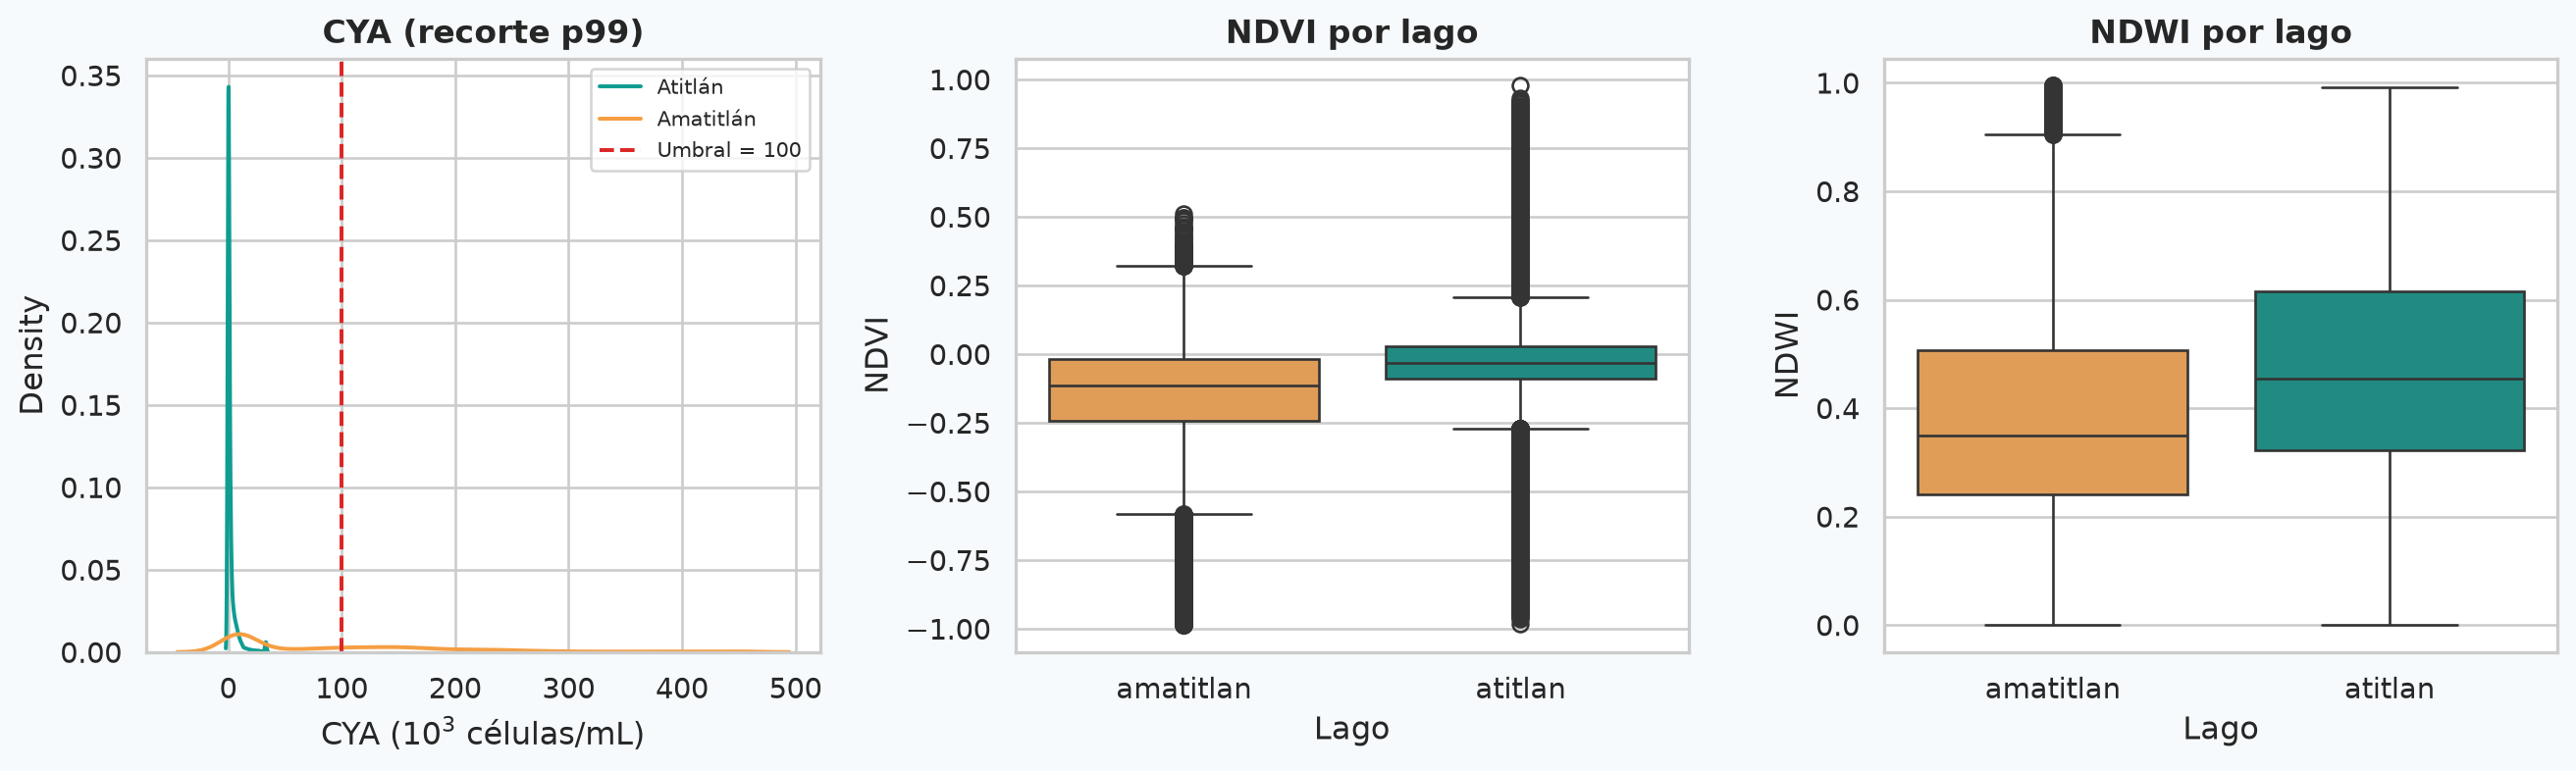
\includegraphics[width=0.78\textwidth]{ml_eda_indices_cya.png}
\caption{Distribuciones y relaciones exploratorias de CYA, NDVI y NDWI.}
\end{figure}

\section{Definición de la respuesta y desbalance}

Se definió $Y=1$ cuando \cya{} $\geq100$, equivalente a 100,000 células/mL. El valor se adoptó como umbral de cribado basado en referencias históricas de la OMS para aguas recreativas. No constituye por sí mismo una declaración toxicológica: Se2WaQ es un proxy óptico transferido y no mide taxonomía, toxinas ni recuentos microscópicos. Una alerta debe confirmarse mediante muestreo de campo.

\begin{table}[H]
\centering
\caption{Distribución completa de la respuesta por lago.}
\begin{tabular}{lrrr}
\toprule
Lago & Baja & Alta & Alta (\%)\\
\midrule
Atitlán & 3,030,910 & 10,842 & 0.36\\
Amatitlán & 215,849 & 161,455 & 42.79\\
\midrule
Global & 3,246,759 & 172,297 & 5.04\\
\bottomrule
\end{tabular}
\end{table}

\begin{figure}[H]
\centering
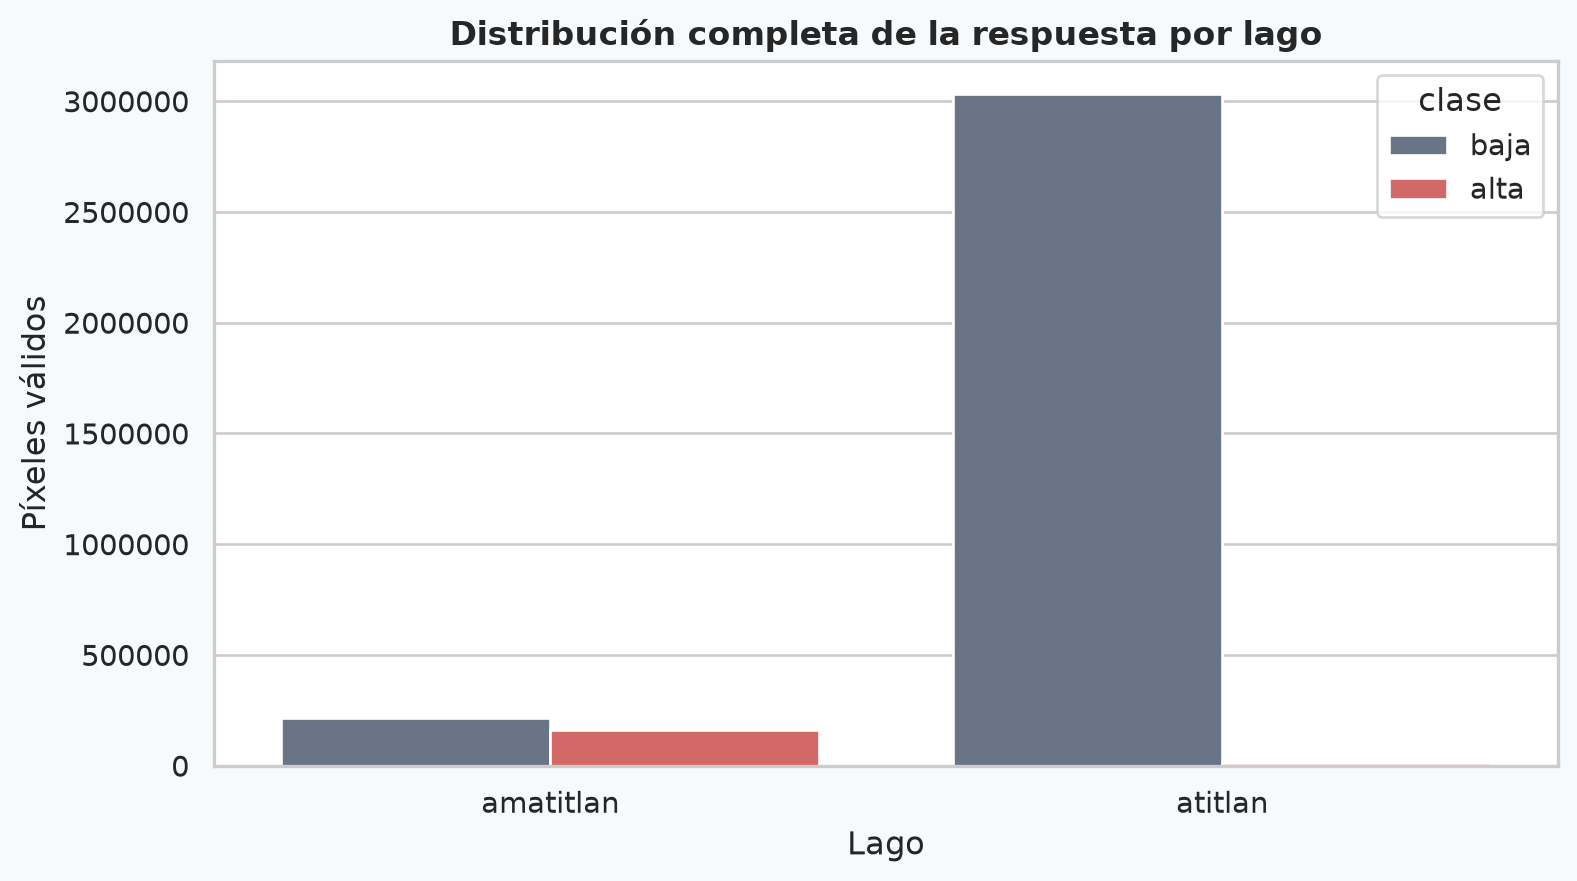
\includegraphics[width=0.67\textwidth]{ml_distribucion_clases.png}
\caption{Desbalance global y diferencias marcadas entre lagos.}
\end{figure}

La prevalencia cambia además entre fechas, como muestra la Figura~\ref{fig:fecha}. Un modelo trivial que prediga siempre ``baja'' alcanzaría accuracy elevada en Atitlán; por ello se reportan precision, recall, F1 y ROC-AUC junto con la matriz de confusión. Desde vigilancia ambiental se prioriza recall: un falso negativo puede omitir una zona que requiere inspección, mientras que un falso positivo aumenta el costo de muestreo, pero todavía permite confirmación.

\begin{figure}[H]
\centering
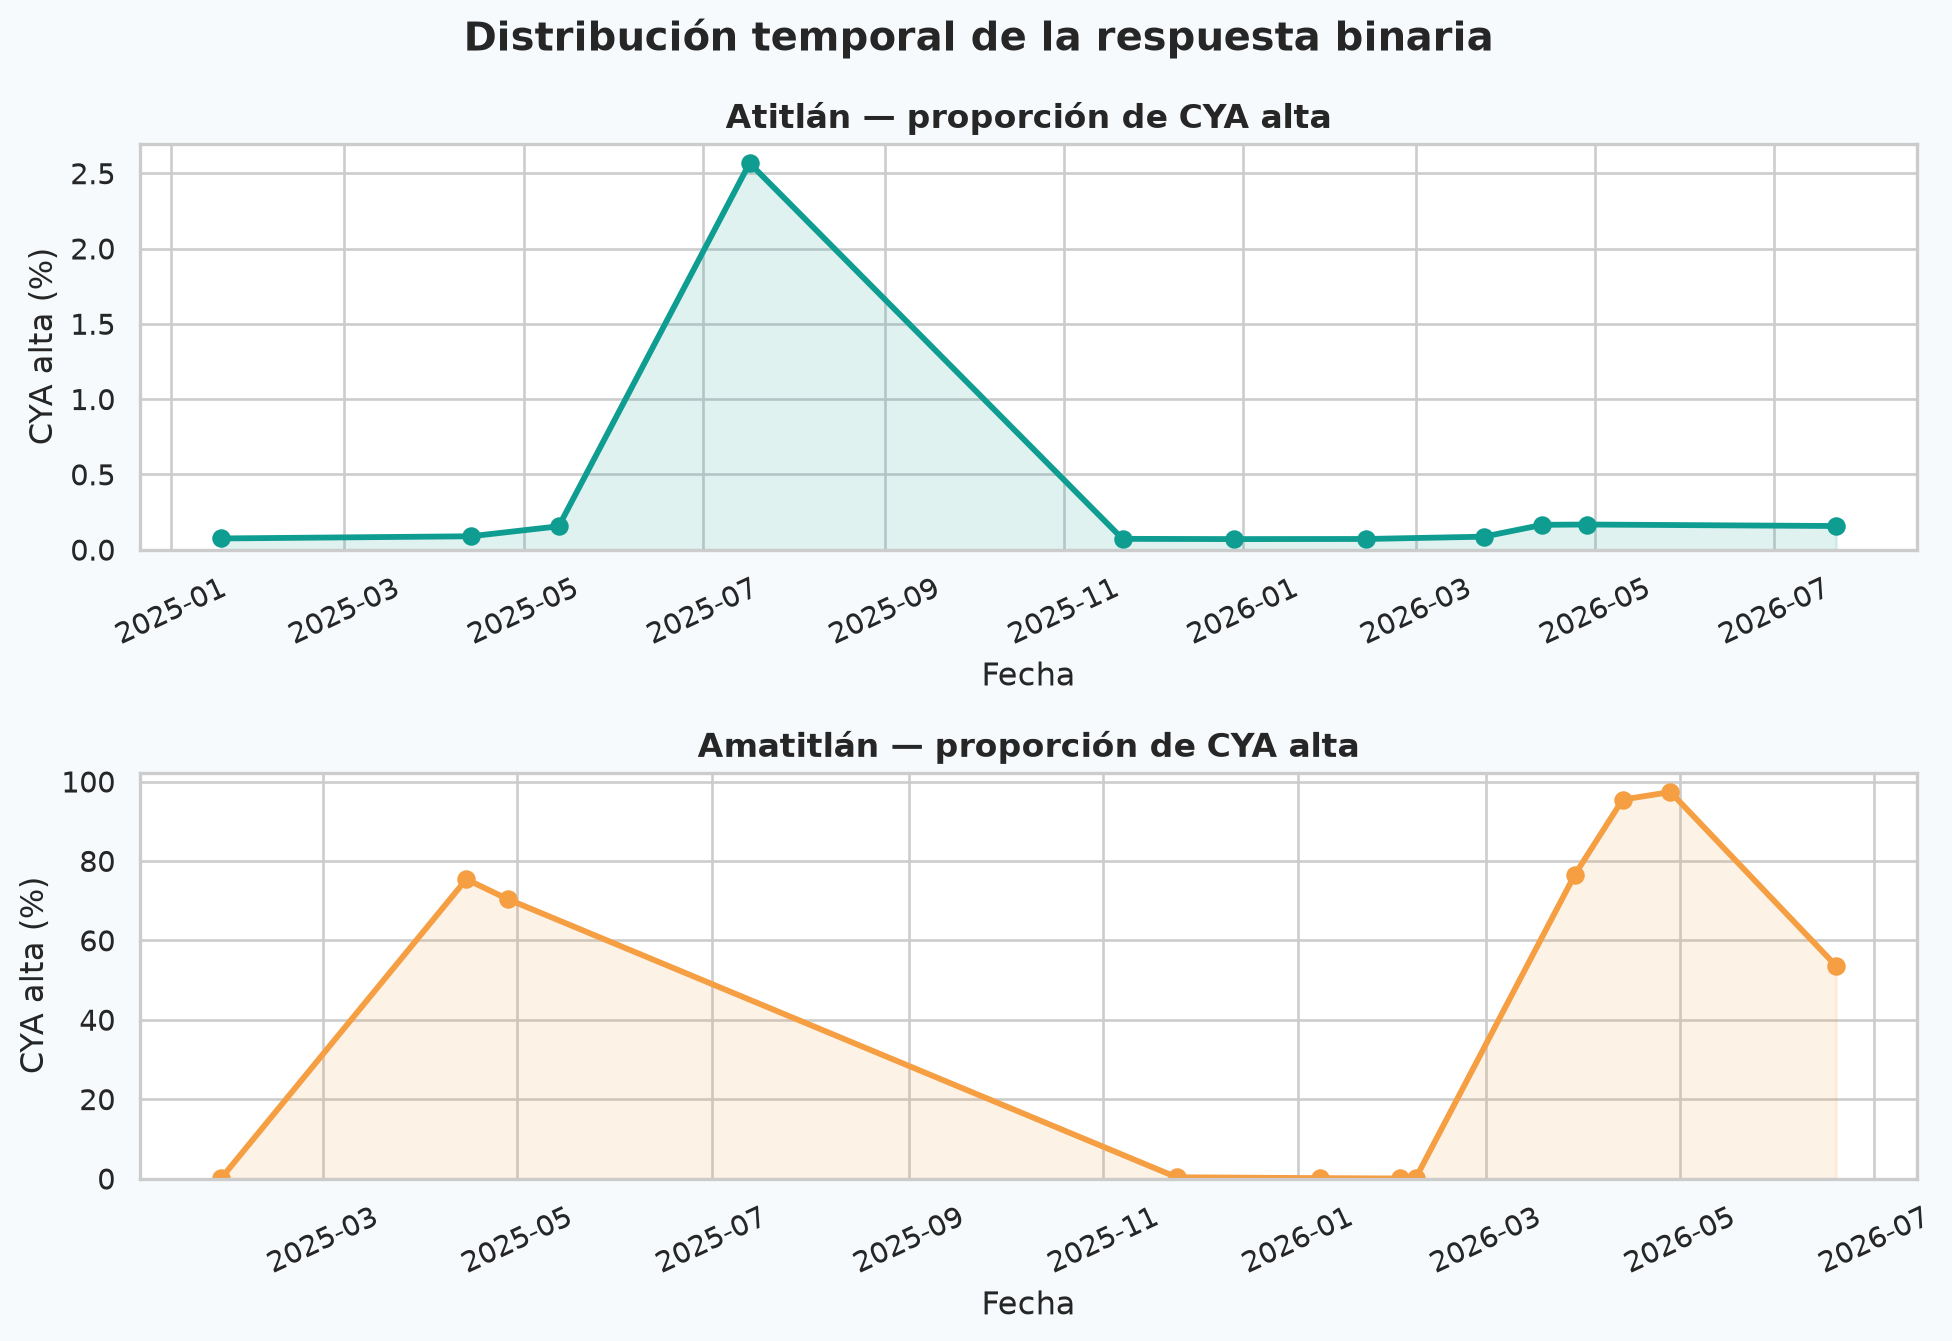
\includegraphics[width=0.96\textwidth]{ml_clases_por_fecha.png}
\caption{Porcentaje y conteo de píxeles de clase alta por lago y fecha.}
\label{fig:fecha}
\end{figure}

\section{Predictores e ingeniería de variables}

La ecuación Se2WaQ usada para la etiqueta es
\[
  \mathrm{CYA}=115530.31\left(\frac{B03\,B04}{B02}\right)^{2.38}.
\]
Se aplicó una exclusión conservadora de fuga de información.

\begin{table}[H]
\centering
\caption{Variables excluidas del entrenamiento.}
\begin{tabularx}{\textwidth}{>{\bfseries}lX}
\toprule
Variable & Motivo\\
\midrule
CYA & Variable continua que define directamente la etiqueta.\\
B02, B03, B04 & Participan directamente en la ecuación del proxy CYA.\\
NDVI & Utiliza B04, que también participa en la construcción de CYA.\\
NDWI & Utiliza B03, que también participa en la construcción de CYA.\\
\bottomrule
\end{tabularx}
\end{table}

Los predictores finales son B05, B06 y B07 (borde rojo), B08 y B8A (infrarrojo cercano), B11 y B12 (infrarrojo de onda corta), coordenadas $x/y$ normalizadas dentro de cada lago y seno/coseno del día del año. Las variables cíclicas evitan la discontinuidad artificial entre diciembre y enero. El nombre del lago no se empleó como predictor, para no entregar al modelo una separación geográfica directa y hacer más honesta la transferencia entre lagos.

\section{Modelos, ajuste y prueba convencional}

Se compararon regresión logística, Random Forest y Gradient Boosting. La partición convencional fue estratificada: 70\% entrenamiento y 30\% prueba. Dentro del entrenamiento, una búsqueda en rejilla con tres pliegues optimizó ROC-AUC sobre hasta 50,000 filas. Después, cada configuración se reajustó con todo el entrenamiento y se evaluó en el mismo conjunto de prueba de 66,000 observaciones.

\begin{table}[H]
\centering
\caption{Hiperparámetros seleccionados.}
\begin{tabularx}{\textwidth}{lXr}
\toprule
Modelo & Configuración & ROC-AUC CV\\
\midrule
Regresión logística & $C=10$, escalamiento y pesos balanceados & 0.9945\\
Random Forest & 120 árboles, profundidad libre, hoja mínima 2 & 0.9983\\
Gradient Boosting & tasa 0.10, 31 hojas, 160 iteraciones & 0.9983\\
\bottomrule
\end{tabularx}
\end{table}

\begin{table}[H]
\centering
\caption{Resultados de la prueba aleatoria común.}
\small
\begin{tabular}{lrrrrr}
\toprule
Modelo & Accuracy & Precision & Recall & F1 & ROC-AUC\\
\midrule
Regresión logística & 0.9670 & 0.8738 & 0.9894 & 0.9280 & 0.9948\\
Random Forest & 0.9838 & 0.9520 & 0.9735 & \textbf{0.9626} & 0.9987\\
Gradient Boosting & 0.9810 & 0.9296 & 0.9865 & 0.9572 & \textbf{0.9987}\\
\bottomrule
\end{tabular}
\end{table}

Random Forest alcanzó el F1 aleatorio más alto por un margen pequeño. Gradient Boosting obtuvo el ROC-AUC máximo y recall alto; se seleccionó como modelo explicativo y cartográfico por ese equilibrio. La regresión logística sacrificó precisión, pero omitió menos positivos.

\begin{figure}[H]
\centering
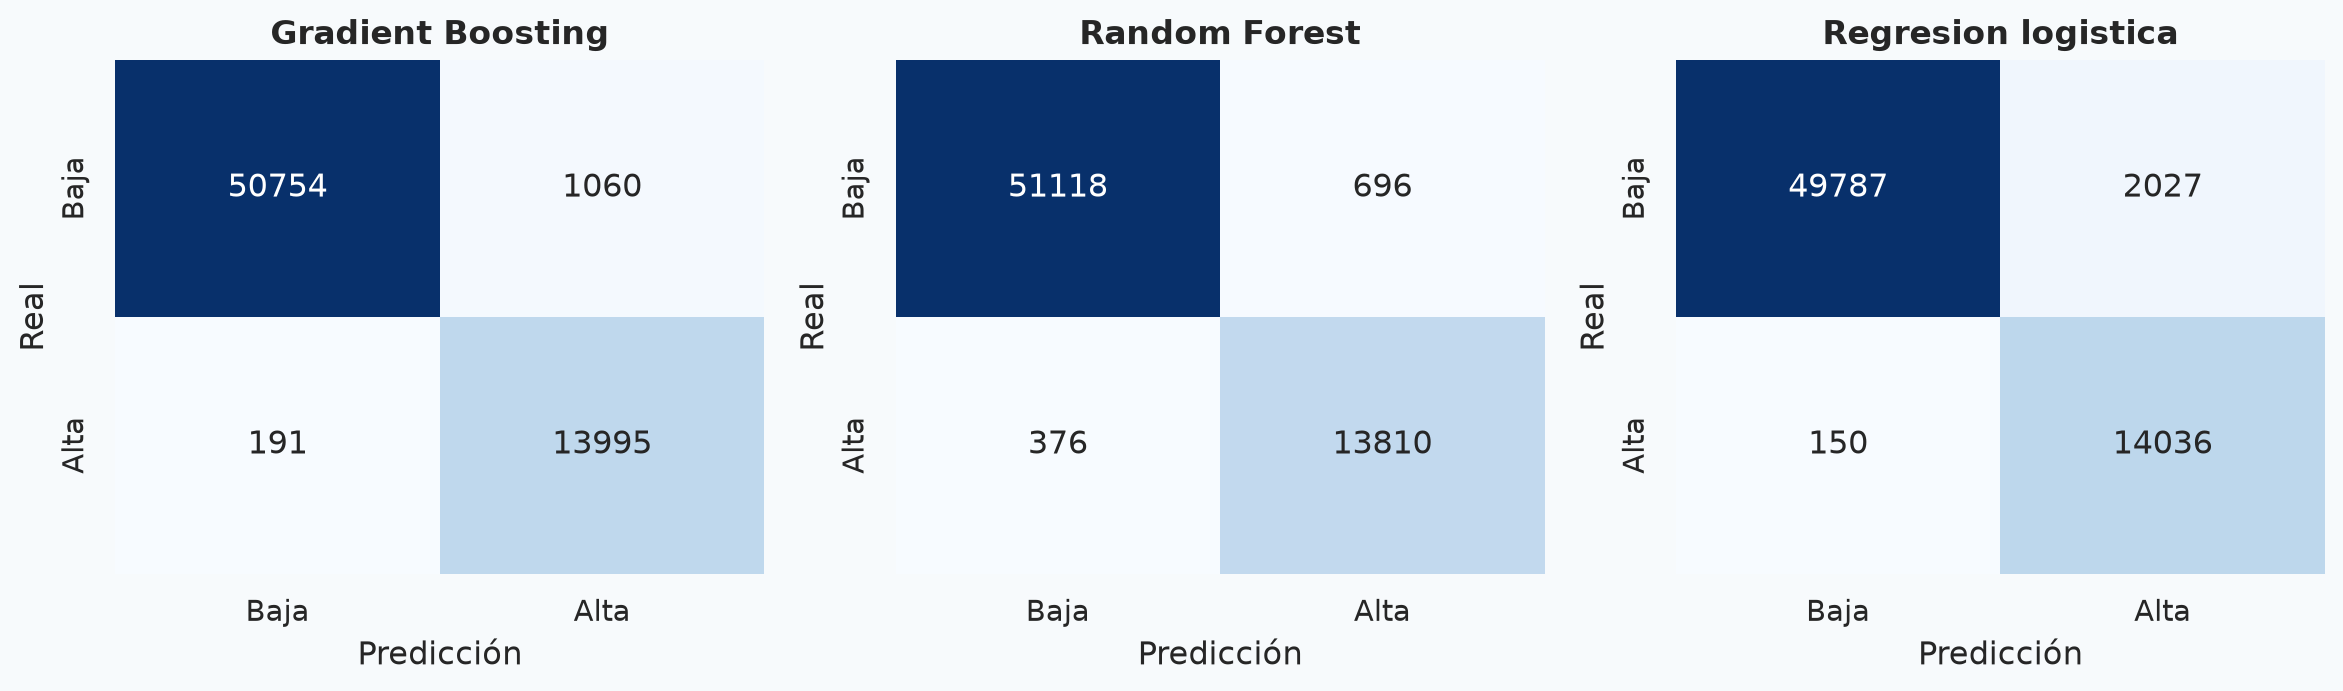
\includegraphics[width=0.92\textwidth]{ml_matrices_confusion_aleatoria.png}
\caption{Matrices de confusión en la prueba aleatoria 70/30.}
\end{figure}

\section{Validación espacial y temporal}

\subsection{Cuadrícula y GroupKFold espacial}

Las coordenadas se expresaron en EPSG:32615 y se asignó cada observación a una cuadrícula de aproximadamente 1 km. Se identificaron 167 bloques con datos en Atitlán y 36 en Amatitlán. GroupKFold de cinco pliegues mantuvo cada bloque completo en entrenamiento o prueba. Así se evita que píxeles del mismo kilómetro aparezcan en ambos conjuntos, aunque bloques vecinos todavía pueden quedar en pliegues distintos.

\begin{figure}[H]
\centering
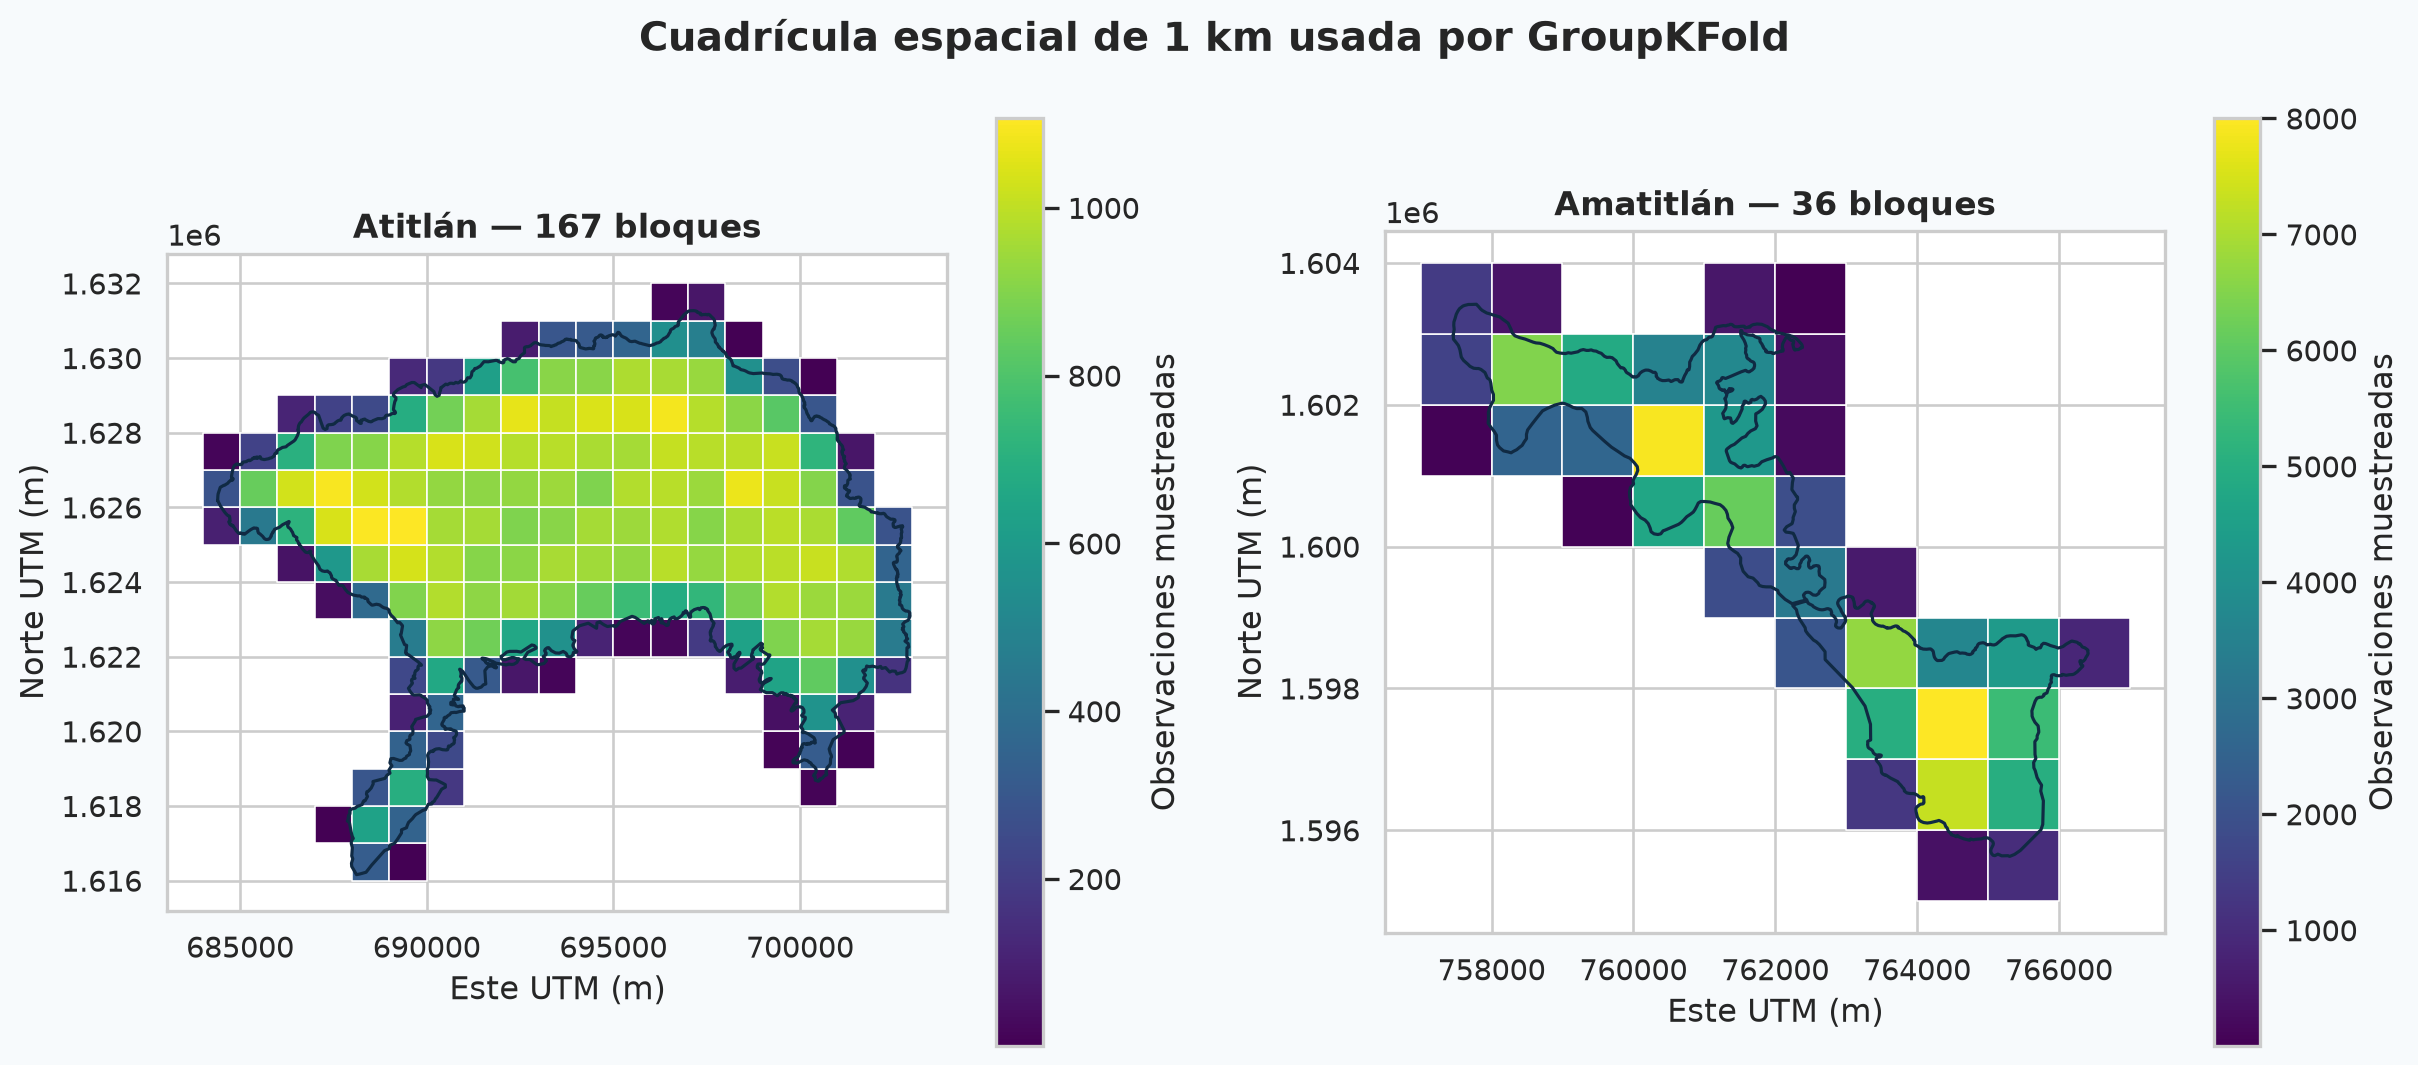
\includegraphics[width=0.94\textwidth]{ml_bloques_espaciales_1km.png}
\caption{Polígonos de la cuadrícula espacial de 1 km y observaciones muestreadas.}
\end{figure}

\subsection{Comparación de escenarios}

La validación temporal retuvo la última fecha completa de cada lago (Atitlán: 22 de julio de 2026; Amatitlán: 19 de junio de 2026) y entrenó exclusivamente con fechas anteriores. Esta prueba mide cambio de distribución y se acerca más al uso prospectivo.

\begin{table}[H]
\centering
\caption{Métricas espaciales y temporales. La fila espacial es el promedio de cinco pliegues.}
\small
\begin{tabular}{llrrrrr}
\toprule
Validación & Modelo & Accuracy & Precision & Recall & F1 & AUC\\
\midrule
Espacial & Logística & 0.9667 & 0.8741 & 0.9863 & 0.9267 & 0.9947\\
Espacial & Random Forest & 0.9818 & 0.9523 & 0.9631 & 0.9576 & 0.9981\\
Espacial & Gradient Boosting & 0.9794 & 0.9274 & 0.9809 & 0.9533 & 0.9982\\
\addlinespace
Temporal & Logística & 0.8700 & 0.6874 & \textbf{0.9384} & \textbf{0.7936} & \textbf{0.9590}\\
Temporal & Random Forest & 0.7765 & 0.9920 & 0.1620 & 0.2785 & 0.9034\\
Temporal & Gradient Boosting & 0.8495 & 0.8164 & 0.5611 & 0.6651 & 0.9080\\
\bottomrule
\end{tabular}
\end{table}

\begin{figure}[H]
\centering
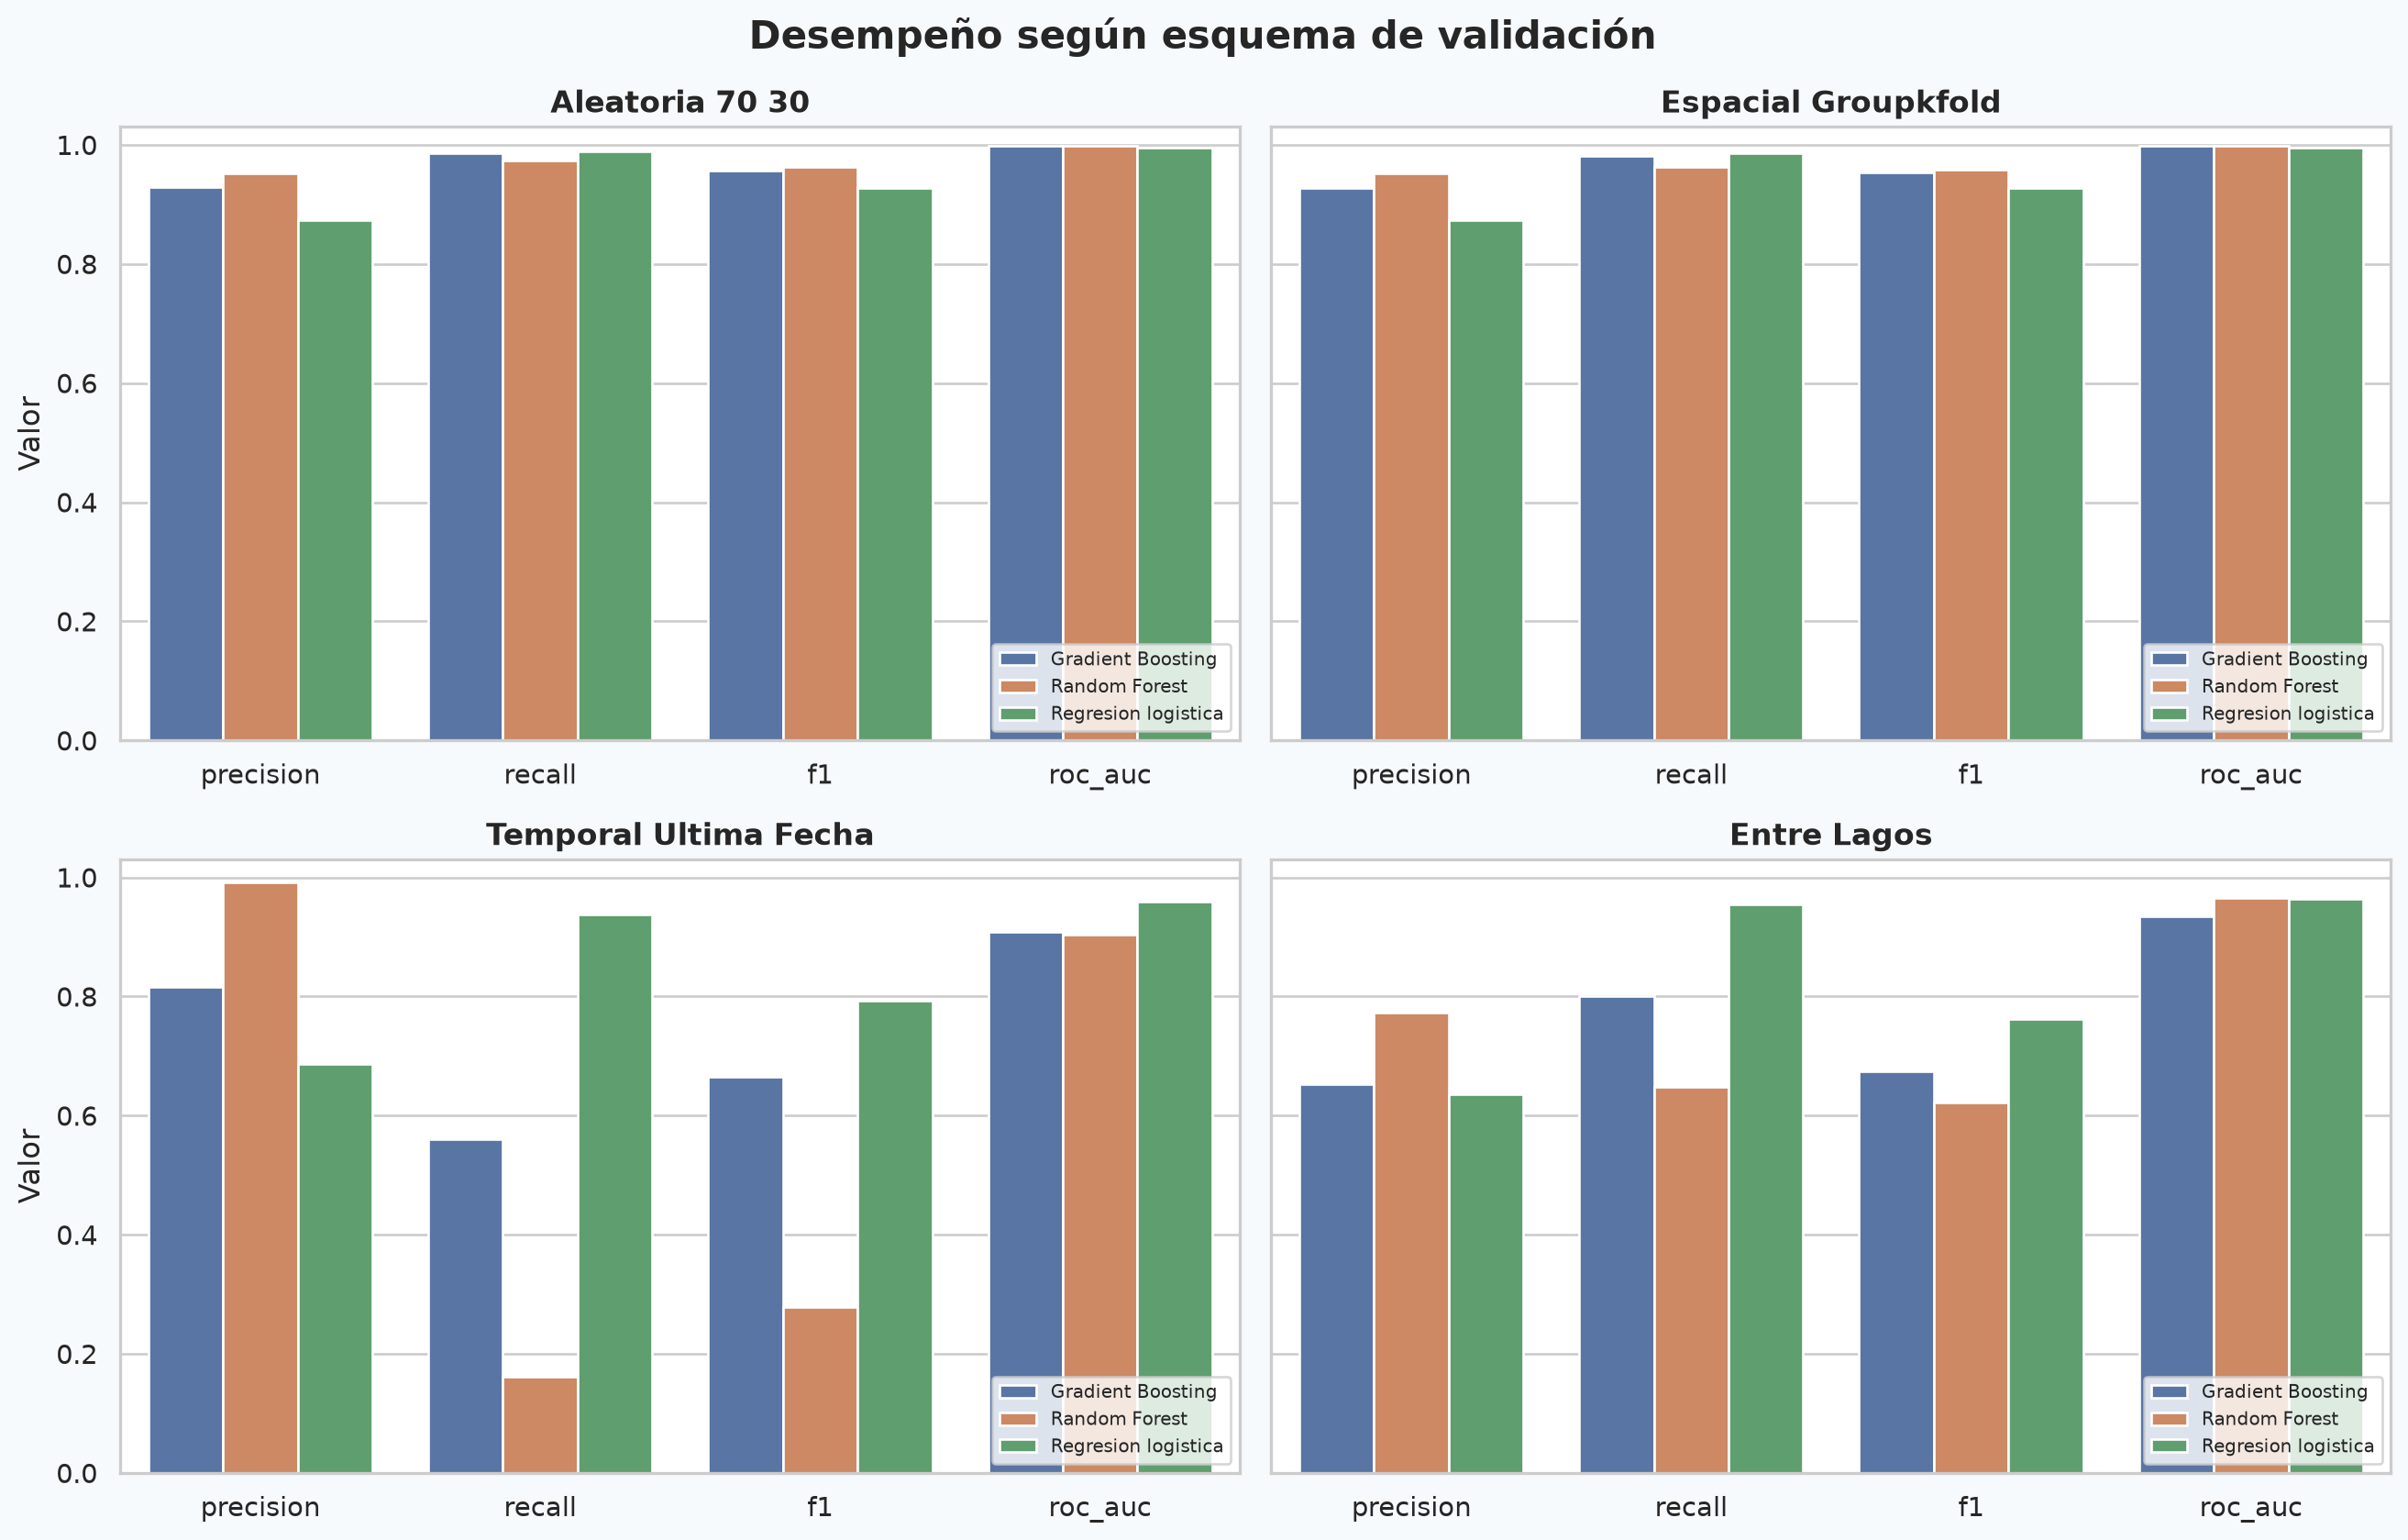
\includegraphics[width=0.96\textwidth]{ml_comparacion_validaciones.png}
\caption{Comparación entre evaluación aleatoria, espacial, temporal y entre lagos.}
\end{figure}

El desempeño espacial cercano al aleatorio indica señal espectral transferible entre los bloques observados. En contraste, la caída temporal es sustancial: Random Forest se vuelve muy conservador y su recall baja a 0.1620; Gradient Boosting pierde 0.2921 puntos de F1 frente a la prueba aleatoria. La regresión logística generaliza mejor en recall temporal. Por tanto, no existe un único ``mejor'' algoritmo sin especificar el costo del error: Gradient Boosting equilibra discriminación y explicación, mientras que la regresión logística es más segura para priorizar no omitir alertas futuras.

\section{Generalización entre lagos}

Cada modelo se entrenó con las 110,000 observaciones muestreadas de un lago y se evaluó sobre las 110,000 del otro, sin reajuste.

\begin{table}[H]
\centering
\caption{Transferencia entre lagos.}
\small
\begin{tabular}{llrrrr}
\toprule
Dirección & Modelo & Precision & Recall & F1 & ROC-AUC\\
\midrule
Atitlán $\rightarrow$ Amatitlán & Logística & 0.691 & 0.960 & 0.804 & 0.930\\
 & Random Forest & 0.964 & 0.364 & 0.529 & 0.938\\
 & Gradient Boosting & 0.865 & 0.658 & 0.747 & 0.869\\
\addlinespace
Amatitlán $\rightarrow$ Atitlán & Logística & 0.580 & 0.951 & 0.721 & 0.998\\
 & Random Forest & 0.580 & 0.932 & 0.715 & 0.994\\
 & Gradient Boosting & 0.441 & 0.943 & 0.601 & 0.999\\
\bottomrule
\end{tabular}
\end{table}

La generalización es asimétrica y peor que la evaluación dentro de la mezcla de ambos lagos. Atitlán aporta solo 0.36\% de positivos, por lo cual entrenar allí ofrece pocos episodios altos y reduce el recall de los modelos de árboles cuando se aplican a Amatitlán. En sentido inverso, los modelos detectan la mayoría de los positivos escasos de Atitlán, pero con precisión moderada. Profundidad, mezcla, altitud, materia suspendida, uso del suelo y presión urbana modifican la firma óptica; un clasificador aprendido en un lago no debe transferirse sin calibración local.

\section{Interpretación del modelo}

\subsection{Importancia global}

La importancia por permutación del Gradient Boosting se midió sobre prueba independiente. B05 produjo la mayor caída del ROC-AUC (0.266), seguida a distancia por B08 y la coordenada norte normalizada. B05 se ubica en el borde rojo, región sensible a cambios de pigmentos y biomasa, pero su asociación es predictiva, no causal: turbidez, profundidad y corrección atmosférica pueden inducir respuestas similares.

\begin{figure}[H]
\centering
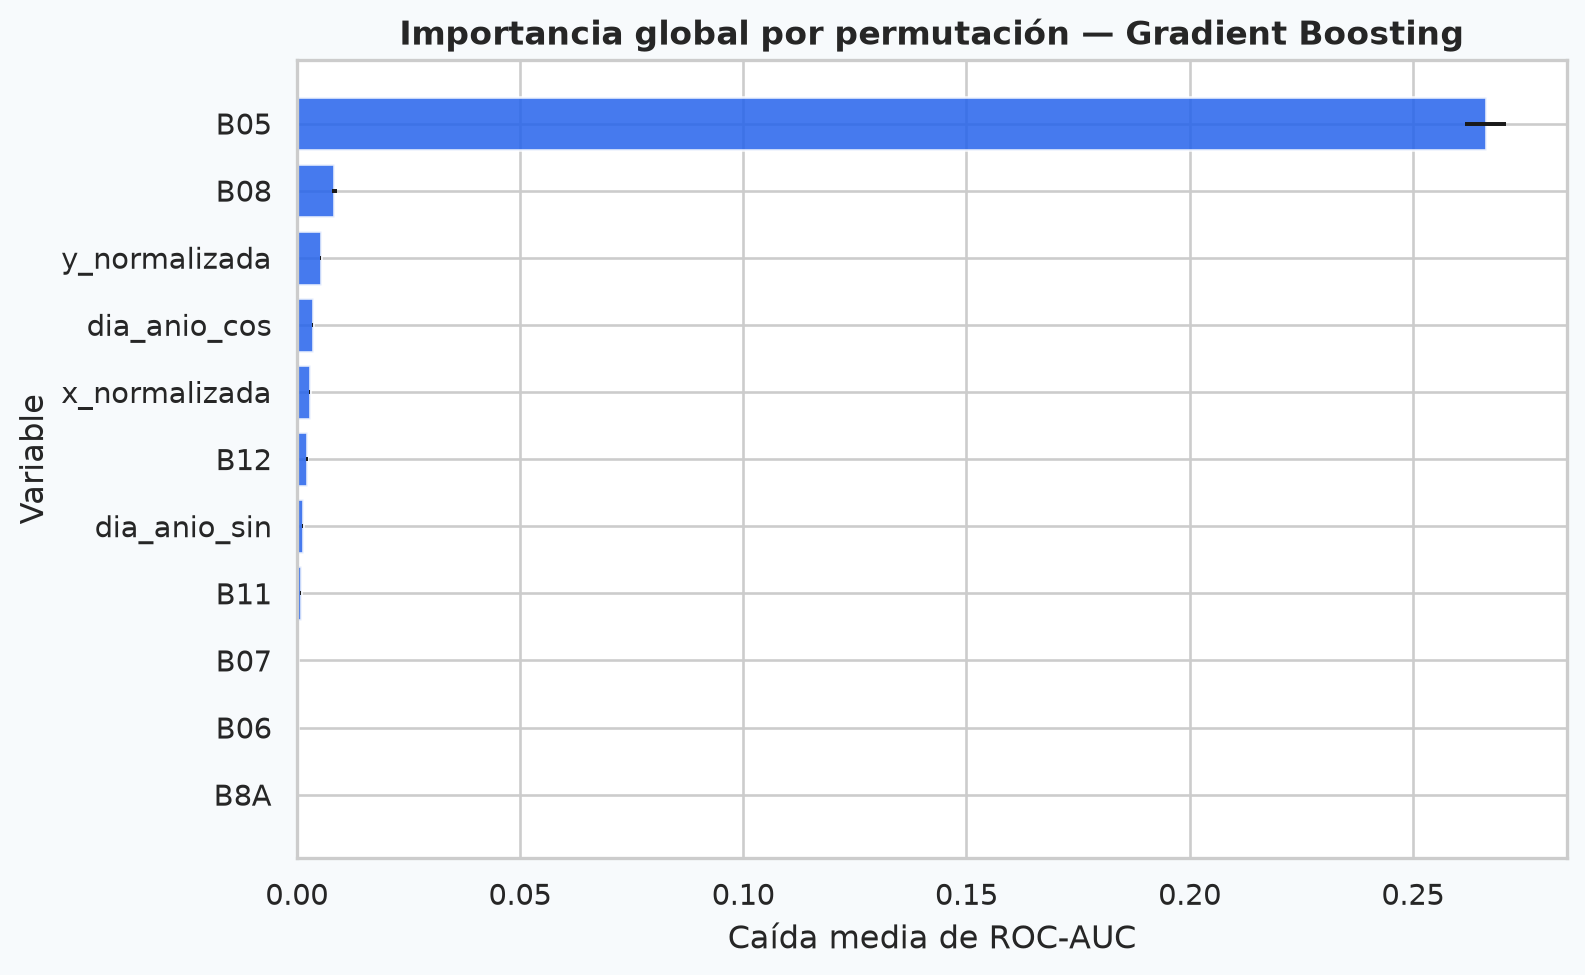
\includegraphics[width=0.70\textwidth]{ml_importancia_global.png}
\caption{Importancia global por permutación.}
\end{figure}

\subsection{SHAP global, dirección y casos locales}

TreeExplainer se aplicó a 4,000 observaciones de prueba del Gradient Boosting. El valor absoluto SHAP promedio confirmó el dominio de B05 (6.916), seguido por B08 (0.995), posición norte (0.340), posición este (0.257) y estacionalidad coseno (0.254). Valores altos de B05, B08, B11 y B12 tienden a aumentar la predicción; B07 y B8A tienden a reducirla. La componente espacial indica heterogeneidad persistente, no causalidad geográfica.

\begin{figure}[H]
\centering
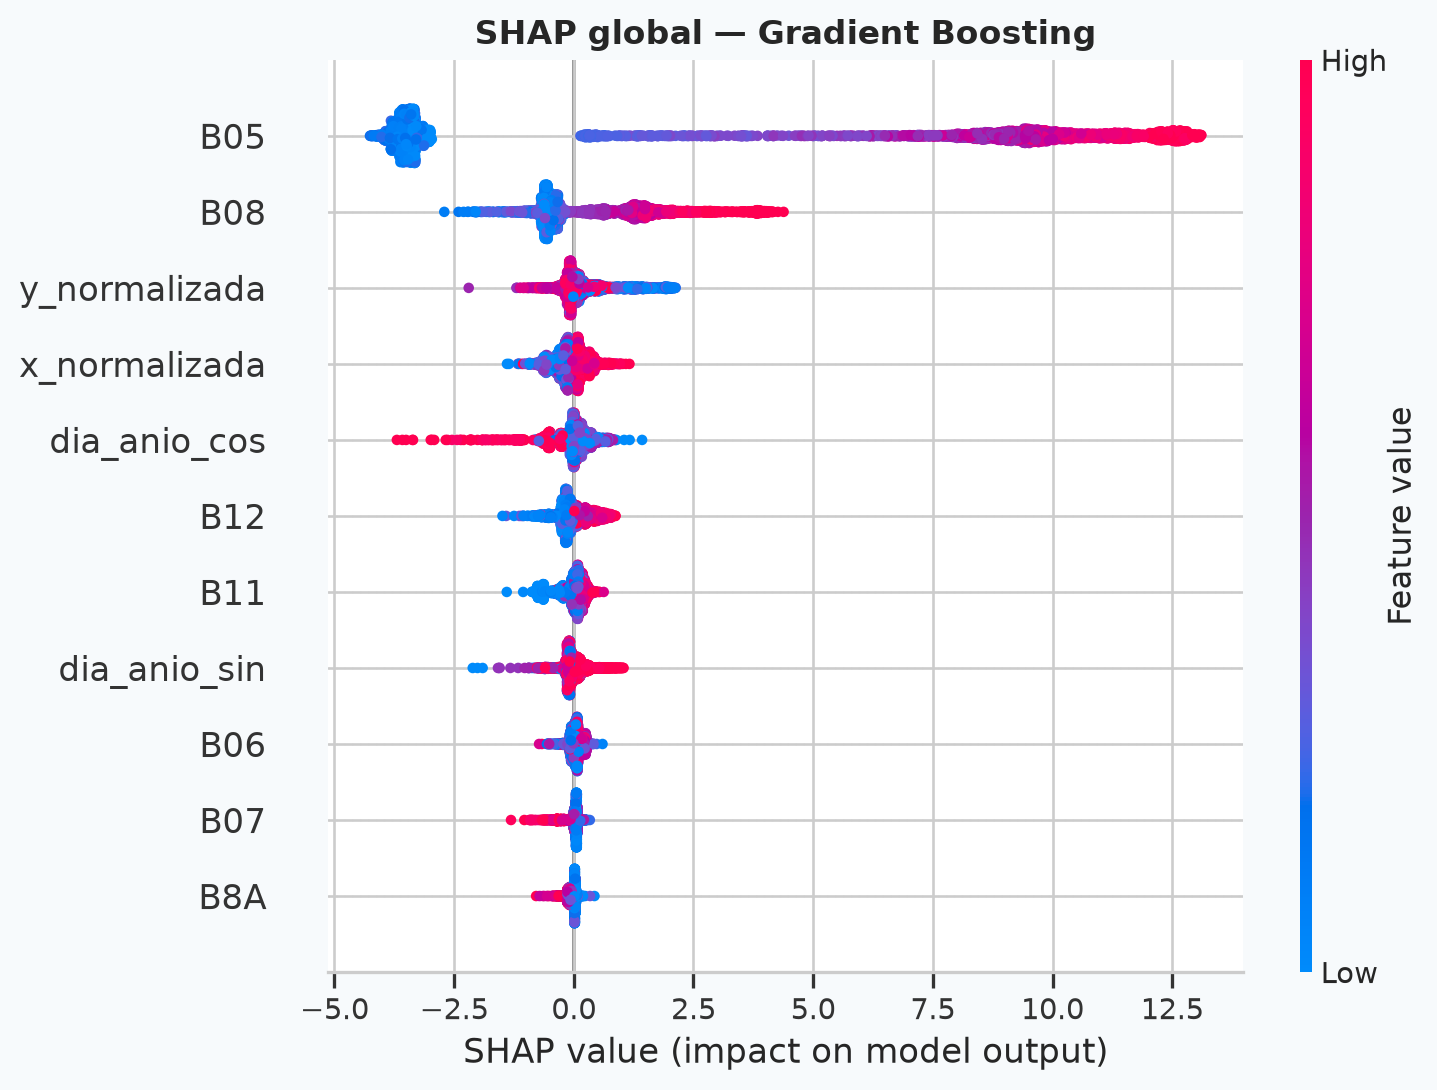
\includegraphics[width=0.92\textwidth]{ml_shap_beeswarm.png}
\caption{Resumen SHAP: magnitud y dirección de los efectos sobre el logit.}
\end{figure}

\begin{figure}[H]
\centering
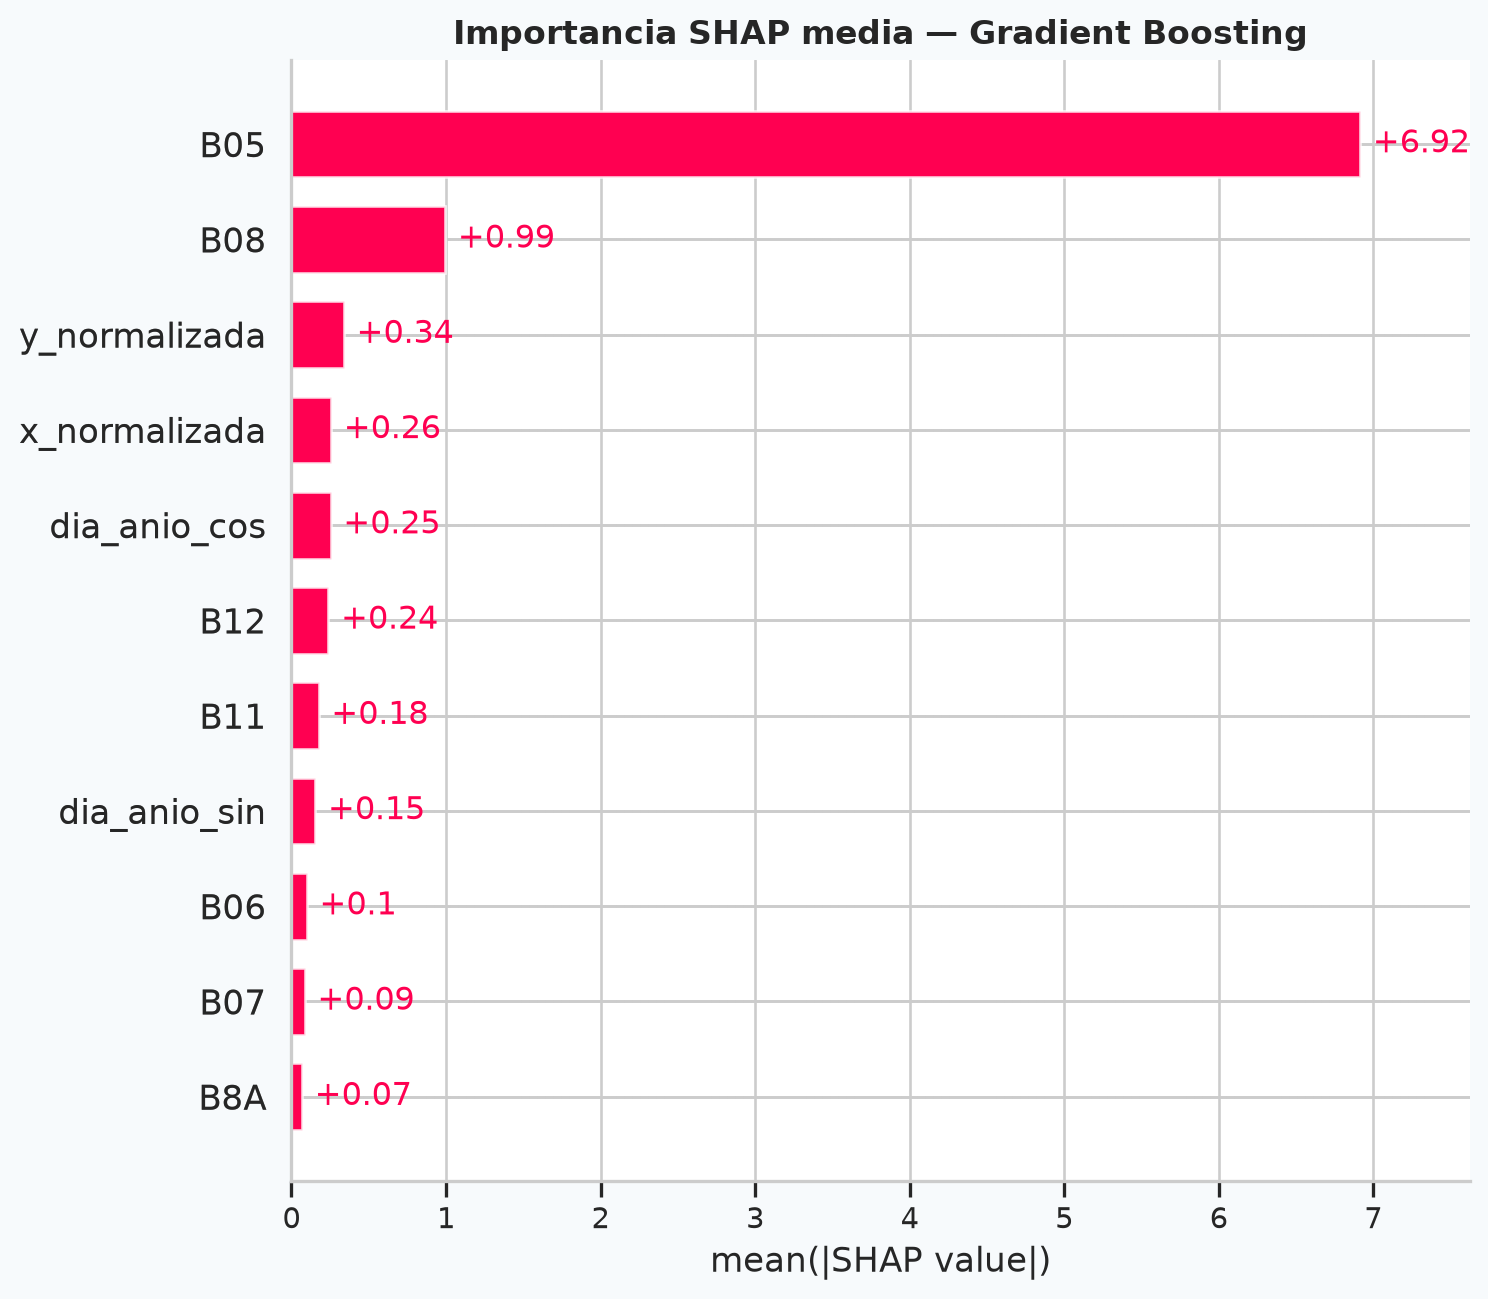
\includegraphics[width=0.82\textwidth]{ml_shap_bar.png}
\caption{Magnitud SHAP media absoluta de los predictores.}
\end{figure}

Las explicaciones locales de una predicción alta y una baja muestran cómo el modelo combina señales: una contribución positiva grande de B05 puede dominar un caso de riesgo, mientras que valores espectrales incompatibles y componentes espaciales negativas sostienen una predicción baja. Estas explicaciones no convierten el modelo en mecanismo biofísico; sirven para auditar consistencia y detectar predicciones sustentadas en variables espurias.

\begin{figure}[H]
\centering
\begin{minipage}{0.49\textwidth}
\centering
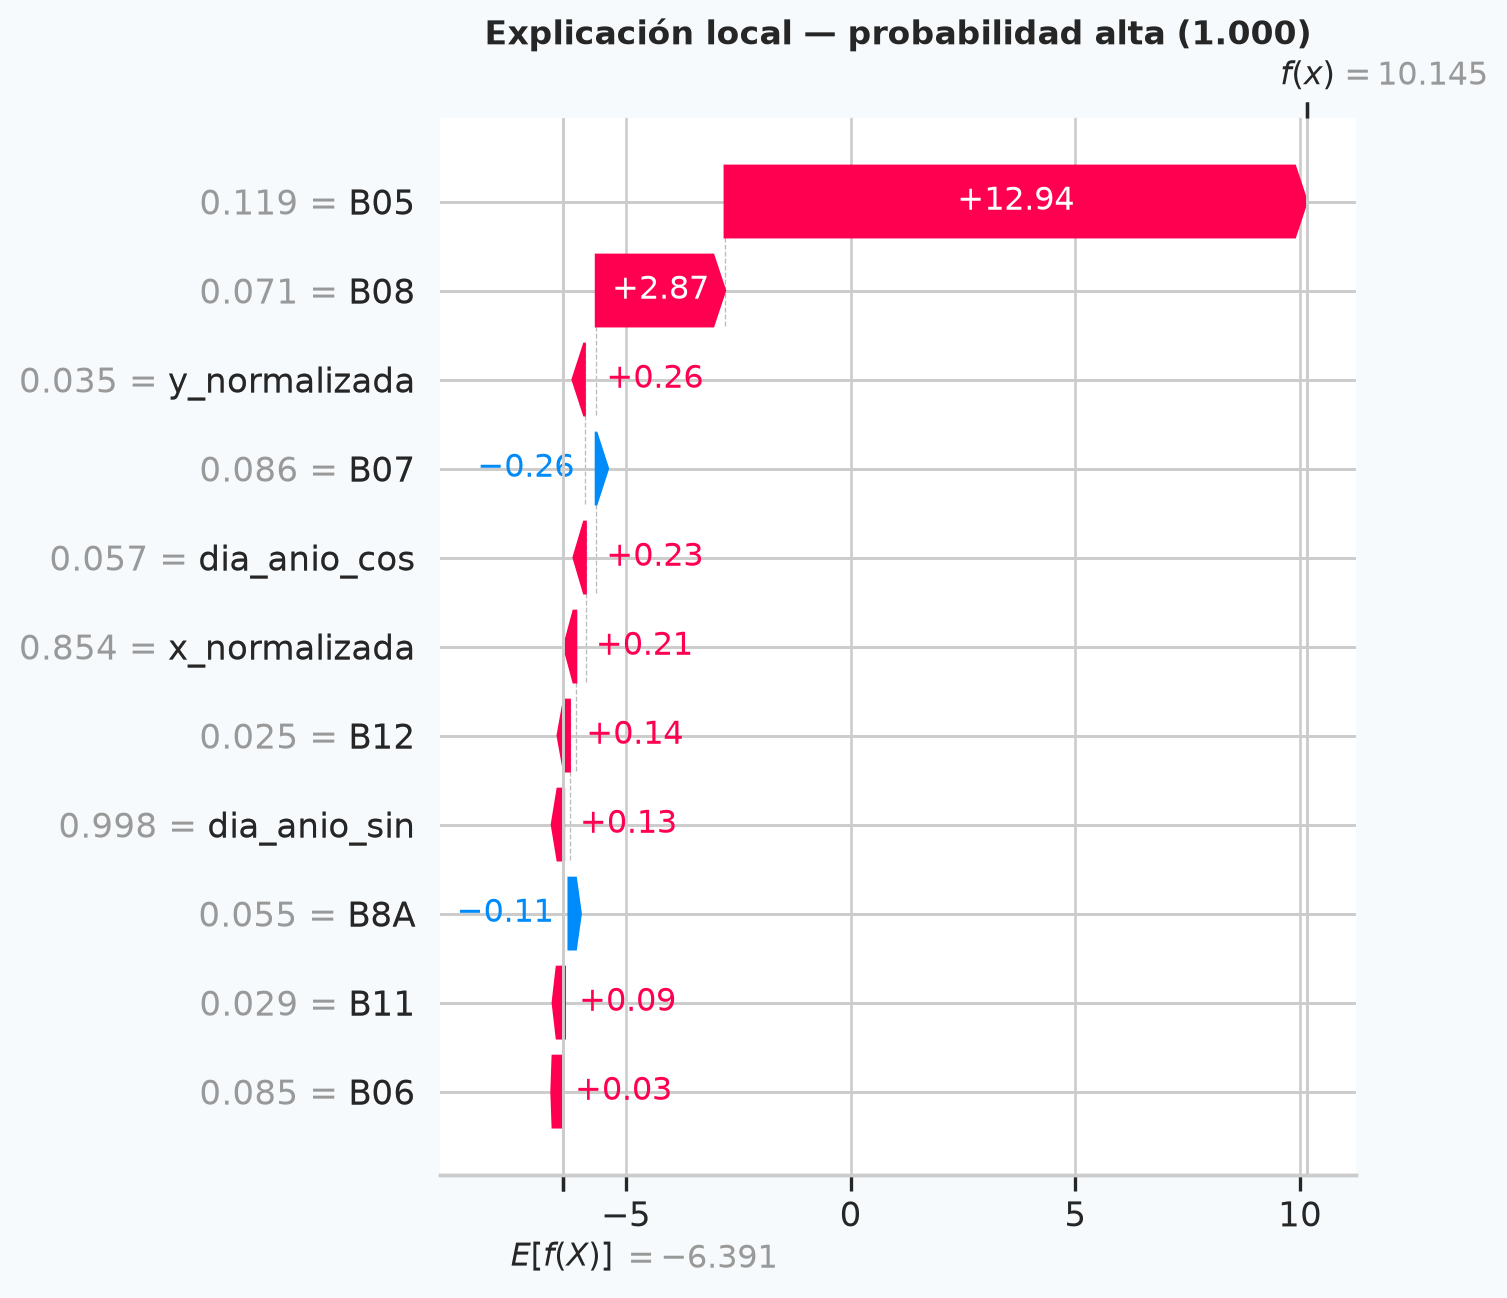
\includegraphics[width=\textwidth]{ml_shap_local_alta.png}
\end{minipage}\hfill
\begin{minipage}{0.49\textwidth}
\centering
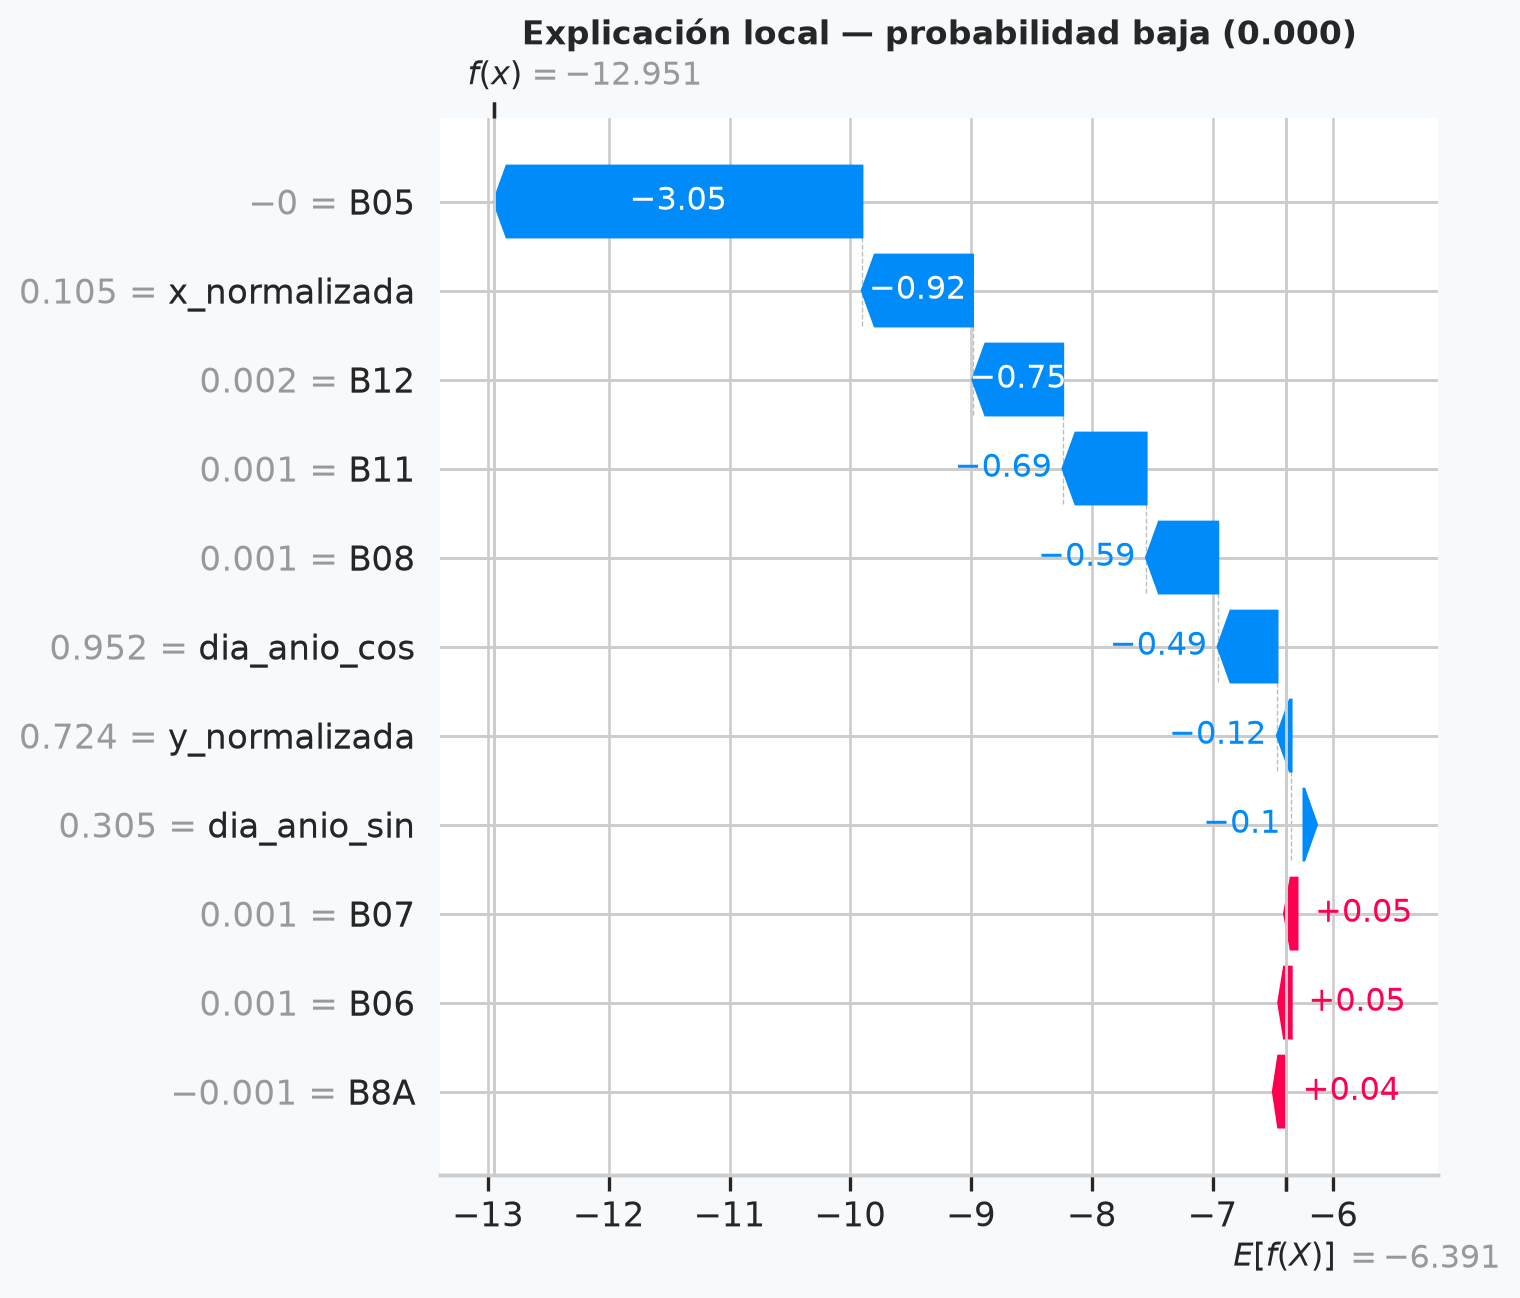
\includegraphics[width=\textwidth]{ml_shap_local_baja.png}
\end{minipage}
\caption{Explicaciones SHAP locales de una predicción alta y una baja.}
\end{figure}

\section{Mapas predictivos y errores espaciales}

El Gradient Boosting final se reajustó sobre la muestra completa únicamente para generar superficies; todas las métricas anteriores permanecen fuera de muestra. Para la última escena de cada lago se predijo cada píxel válido y se clasificó la probabilidad en baja ($p<0.30$), media ($0.30\leq p<0.70$) y alta ($p\geq0.70$). Las categorías representan confianza del modelo, no nuevos umbrales sanitarios.

\begin{table}[H]
\centering
\caption{Resumen de mapas predictivos de la última fecha.}
\small
\begin{tabular}{lrrrrr}
\toprule
Lago & Píxeles & $\bar p$ & Baja (\%) & Media (\%) & Alta (\%)\\
\midrule
Atitlán, 2026-07-22 & 301,570 & 0.003 & 99.77 & 0.07 & 0.16\\
Amatitlán, 2026-06-19 & 34,483 & 0.623 & 31.73 & 8.70 & 59.58\\
\bottomrule
\end{tabular}
\end{table}

\begin{figure}[H]
\centering
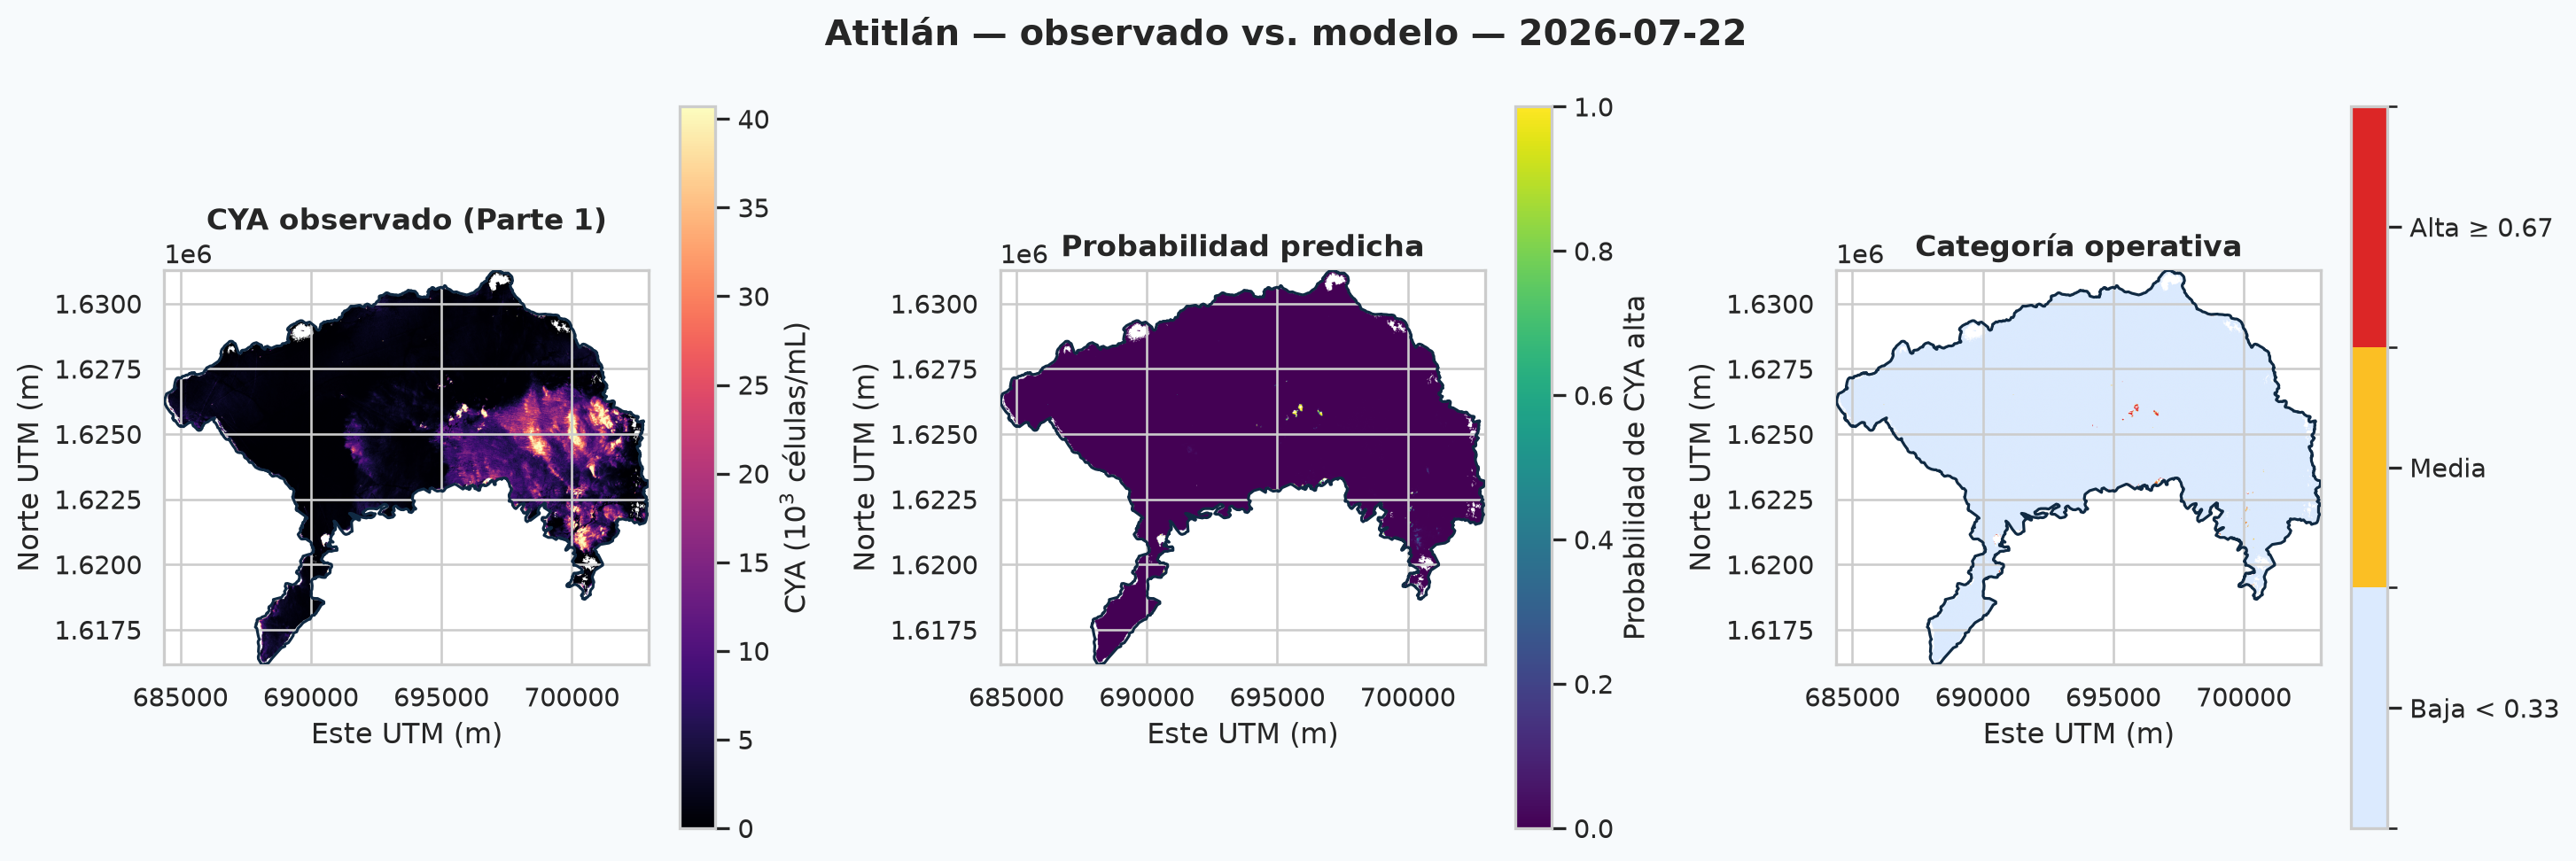
\includegraphics[width=0.98\textwidth]{ml_comparacion_observado_predicho_atitlan.png}
\caption{Atitlán: CYA observado, probabilidad y categoría predictiva.}
\end{figure}

\begin{figure}[H]
\centering
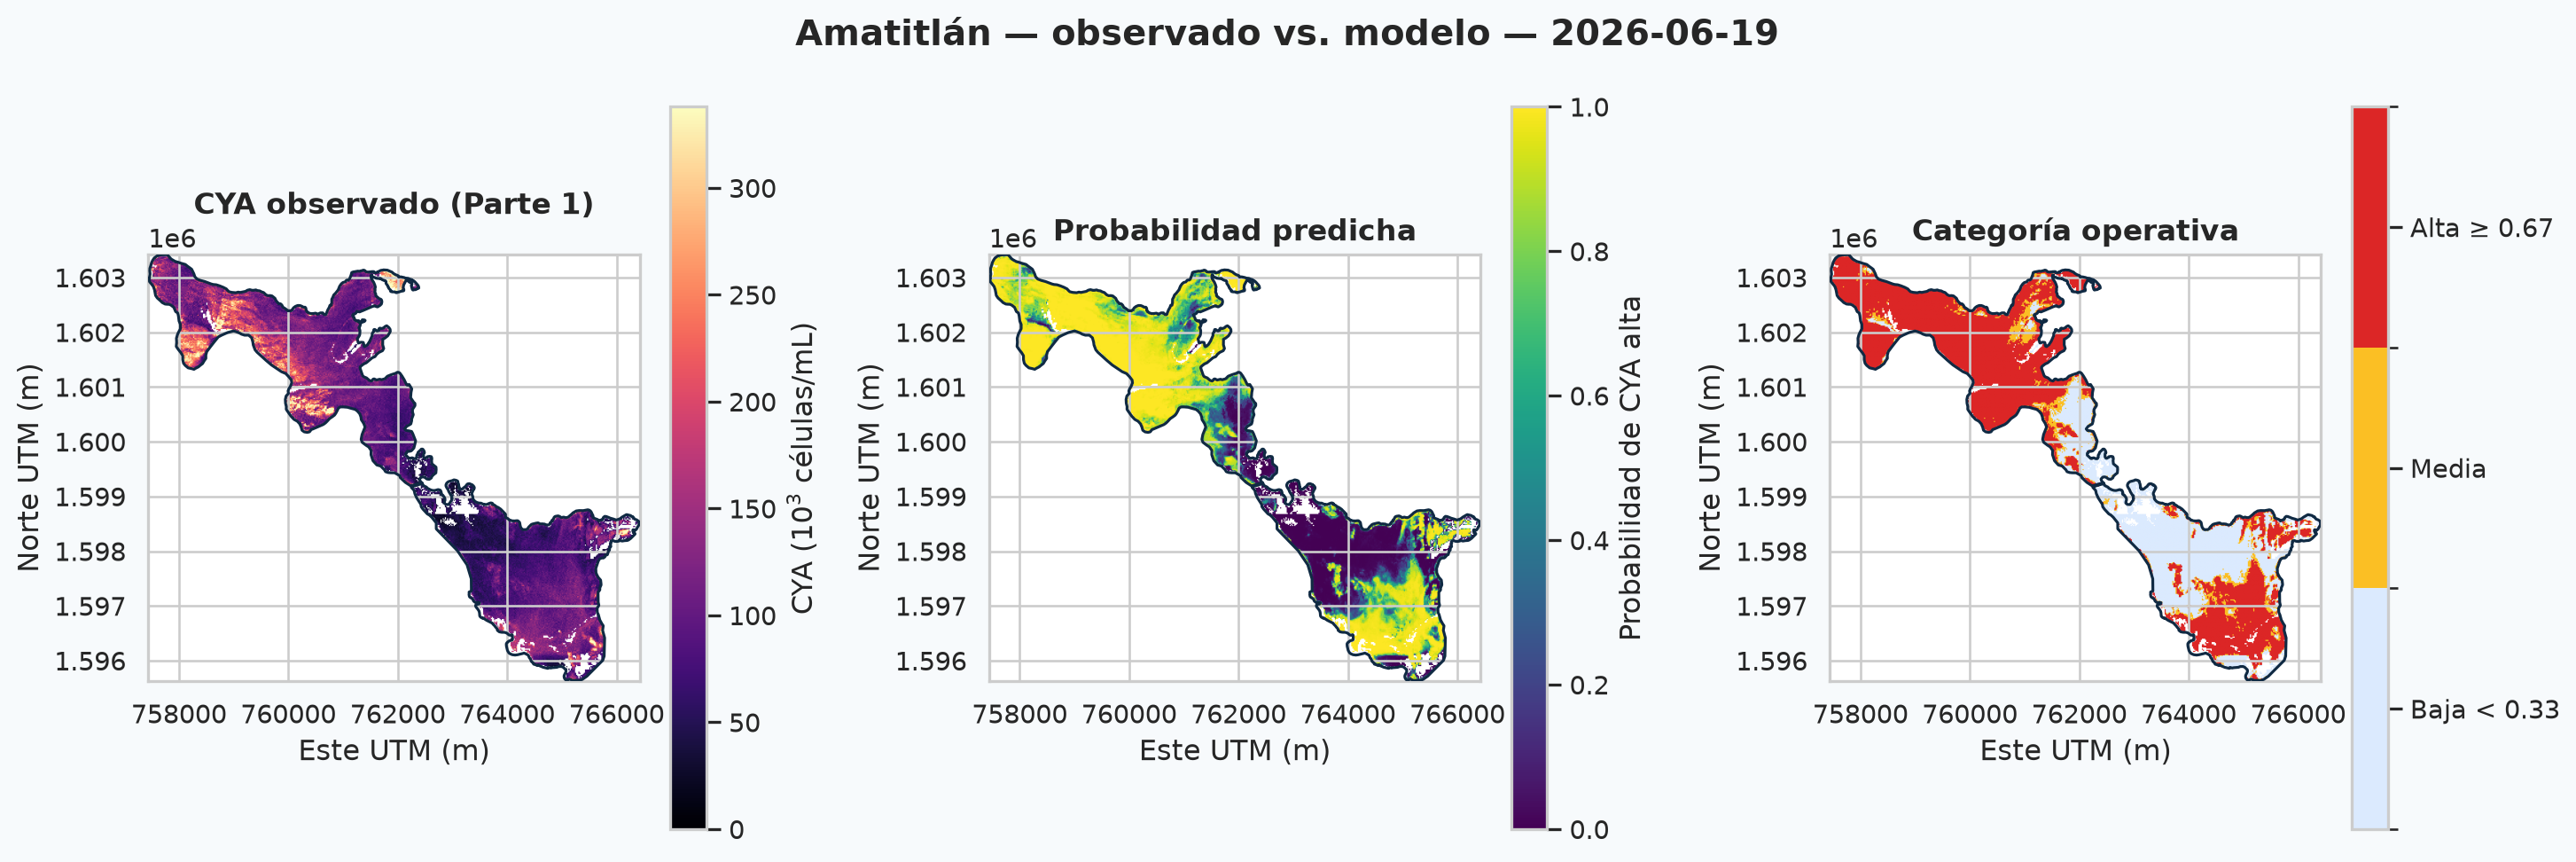
\includegraphics[width=0.98\textwidth]{ml_comparacion_observado_predicho_amatitlan.png}
\caption{Amatitlán: CYA observado, probabilidad y categoría predictiva.}
\end{figure}

Los mapas son coherentes con la Parte 1: la escena final de Atitlán presenta concentración baja casi generalizada, mientras que Amatitlán mantiene un patrón amplio de riesgo alto. La comparación no es una validación independiente, porque la clase observada proviene del mismo proxy remoto; su utilidad es verificar concordancia espacial y priorizar puntos de muestreo.

Los errores cartografiados proceden de predicciones fuera de muestra de los cinco pliegues espaciales de Gradient Boosting. En la muestra de 220,000 filas hubo 3,640 falsos positivos y 889 falsos negativos; Amatitlán concentró 862 FN y 3,572 FP, mientras Atitlán tuvo 27 FN y 68 FP. Los errores se agrupan en transiciones y zonas heterogéneas, donde mezcla de píxel, borde de agua, turbidez o cambio temporal pueden alterar la señal.

\begin{figure}[H]
\centering
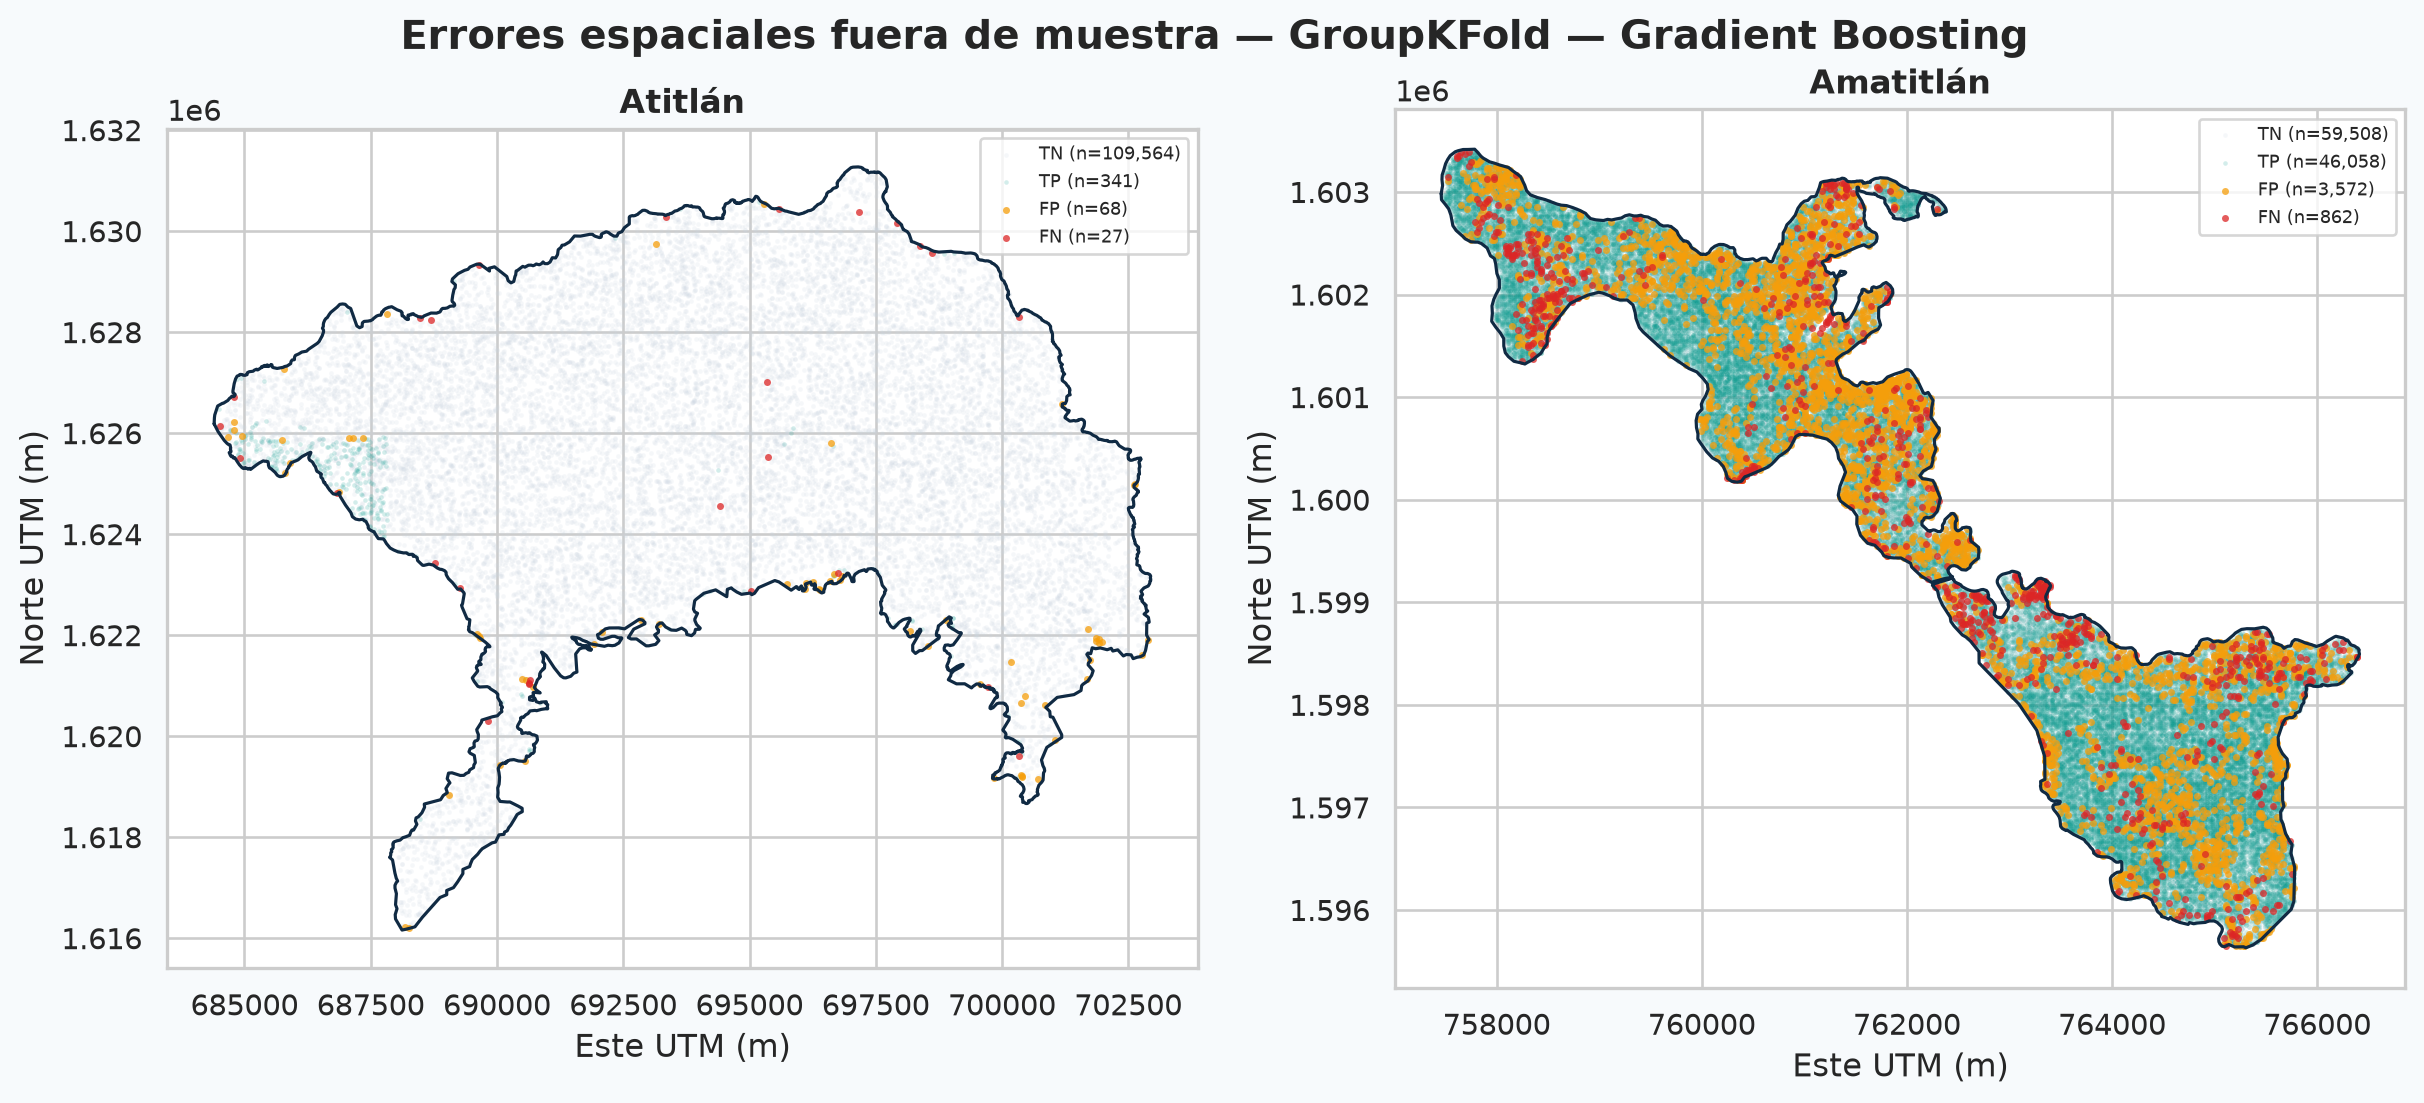
\includegraphics[width=0.98\textwidth]{ml_errores_espaciales.png}
\caption{Verdaderos y falsos resultados fuera de muestra bajo GroupKFold espacial.}
\end{figure}

\section{Conclusiones, utilidad y limitaciones}

\begin{enumerate}
\item Es posible clasificar el proxy CYA con señal espectral que no interviene directamente en su fórmula. El control de fuga evita una solución circular y hace que las métricas reflejen generalización entre bandas independientes.
\item La prueba aleatoria es optimista para uso operativo. La validación temporal reveló degradación fuerte, en especial del recall de Random Forest. Cualquier despliegue requiere monitorear cambio de distribución y reentrenar con campañas nuevas.
\item La validación espacial fue estable dentro de la cobertura estudiada, pero la transferencia entre lagos fue asimétrica. Se recomienda calibración por lago y conservar evaluación separada por cuerpo de agua.
\item B05 y B08 dominan la explicación del Gradient Boosting. Esto es compatible con sensibilidad del borde rojo y NIR a propiedades ópticas del agua, pero SHAP no establece causalidad ni distingue por sí solo cianobacterias de sedimentos u otros pigmentos.
\item Como herramienta ambiental, el sistema sirve para ordenar recorridos, localizar zonas persistentes y priorizar muestras. Si el objetivo es minimizar eventos omitidos, la regresión logística ofrece el recall temporal más favorable; si se busca discriminación global y cartografía, Gradient Boosting ofrece un mejor balance.
\end{enumerate}

Las principales limitaciones son: respuesta derivada de un proxy y no de verdad de campo; solo once fechas por lago; autocorrelación residual entre bloques vecinos; nubes y geometría de adquisición; resolución de 20 m; mezcla en orillas; fuerte diferencia de prevalencia; y evaluación limitada a dos lagos guatemaltecos. Los umbrales de probabilidad no están calibrados como niveles sanitarios.

Para fortalecer el modelo se necesitan conteos celulares y taxonómicos georreferenciados, clorofila-a, ficocianina y toxinas; temperatura, pH, oxígeno disuelto, turbidez, transparencia y nutrientes; profundidad y batimetría; viento y precipitación acumulada; descargas, uso del suelo y tratamiento de aguas; más fechas y años, incluyendo estación lluviosa y seca; y sensores complementarios o productos atmosféricos. Una siguiente evaluación debería usar campañas prospectivas, bloques espaciales contiguos y calibración explícita de probabilidades.

\section{Reproducibilidad y entregables}

El repositorio contiene el notebook final ejecutado, el informe en \LaTeX{} y PDF, el código modular, las pruebas automatizadas, las tablas y figuras. Los 22 GeoTIFF y productos derivados de gran tamaño se mantienen fuera de Git mediante \code{.gitignore}; pueden regenerarse con los scripts documentados. Las credenciales de Copernicus nunca se escriben en archivos: la descarga usa autenticación por código de dispositivo.

\section*{Referencias}

\begin{enumerate}
\item World Health Organization. \emph{Guidelines on recreational water quality: Volume 1, coastal and fresh waters}. 2021. \url{https://www.who.int/publications/i/item/9789240031302}
\item U.S. Environmental Protection Agency. \href{https://www.epa.gov/habs/world-health-organization-who-1999-guideline-values-cyanobacteria-freshwater}{\emph{WHO 1999 Guideline Values for Cyanobacteria in Freshwater}.}
\item Sentinel Hub. \emph{Se2WaQ -- Sentinel-2 Water Quality}. \url{https://custom-scripts.sentinel-hub.com/custom-scripts/sentinel-2/se2waq/}
\item Copernicus Data Space Ecosystem. \emph{openEO API}. \url{https://openeo.dataspace.copernicus.eu/}
\item Lundberg, S. M. y Lee, S.-I. \href{https://proceedings.neurips.cc/paper/2017/hash/8a20a8621978632d76c43dfd28b67767-Abstract.html}{\emph{A Unified Approach to Interpreting Model Predictions}. NeurIPS, 2017.}
\end{enumerate}

\end{document}
